\documentclass[11pt]{article}

% basic packages
\usepackage[margin=1in]{geometry}
\usepackage[pdftex]{graphicx}
\usepackage{amsmath,amssymb,amsthm}
\usepackage{william}
\usepackage{tikz}

% page formatting
\usepackage{fancyhdr}
\pagestyle{fancy}
\renewcommand{\sectionmark}[1]{\markright{\textsf{\arabic{section}. #1}}}
\renewcommand{\subsectionmark}[1]{}
\lhead{\textbf{\thepage} \ \ \nouppercase{\rightmark}}
\chead{}\rhead{}\lfoot{}\cfoot{}\rfoot{}
\setlength{\headheight}{14pt}

\linespread{1.04}
\setlength{\parindent}{0.2in}
\setcounter{secnumdepth}{3}
\setcounter{tocdepth}{2}

% ---- local macros for this explainer ----
\newcommand{\supp}{\operatorname{supp}}
\newcommand{\dd}{\mathrm{d}}                 % exterior derivative
\newcommand{\Pexp}{\mathcal{P}\!\exp}        % path-ordered exponential
\newcommand{\half}{\tfrac12}
\DeclareMathOperator{\Hol}{Hol}              % holonomy
\newcommand{\Uone}{\mathrm{U}(1)}
\newcommand{\SUN}{\mathrm{SU}(N)}
\newcommand{\Ztwo}{\mathbb{Z}_2}
\newcommand{\ZN}{\mathbb{Z}_N}
% green "Exercise" box, reusing the green-box style from william.sty
\declaretheorem[style=thmgreenbox,name=Exercise,numberwithin=section]{xca}

\begin{document}

\thispagestyle{empty}
\bigskip
\vspace{0.1cm}
\begin{center}
{\fontsize{20}{20} \selectfont An Explainer on}
\vskip 14pt
{\fontsize{34}{34} \selectfont \bf \sffamily Gauge Fields}
\vskip 10pt
{\fontsize{16}{16}\selectfont \sffamily From connections to the modern point of view}
\vskip 22pt
{\fontsize{16}{16} \selectfont \rmfamily \href{https://will-lancer.github.io}{Will Lancer}}
\vskip 6pt
{\fontsize{12}{12} \selectfont \ttfamily will.m.lancer@gmail.com}
\vskip 18pt
\end{center}

{\parindent0pt \baselineskip=15.5pt}
\noin
These notes are an attempt to fully decode statements like ``$A$ is a $\Uone$-gauge
field,'' ``$\mu$ is a $\Ztwo$-gauge field,'' and ``$a$ is a background gauge field for
the global symmetry $G$.'' We start from the physics you already know (Maxwell, the
covariant derivative, Aharonov--Bohm), build up to the geometric definition
(a gauge field is a \emph{connection} on a \emph{principal bundle}), make sense of
\emph{finite}-group gauge fields (which have no Lie algebra), and then turn to the
distinction between \vocab{background} and \vocab{dynamical} gauge fields. That
distinction is the doorway to the modern, ``Seiberg-style'' point of view, in which a
quantum field theory is understood through how its symmetries couple to background
fields, what happens when you \vocab{gauge} them, and what obstructs gauging
(\vocab{'t Hooft anomalies}). We close with a working preview of generalized
(higher-form) global symmetries.

\medskip
\noin
\emph{Prerequisites.} A first course in QFT (path integrals, Noether's theorem), basic
Lie groups/algebras, and enough differential geometry to be unafraid of differential
forms. No bundle theory is assumed; we build what we need.

\medskip
\noin
\emph{How to read.} Boxes labelled \textsf{Definition}/\textsf{Theorem} are the
load-bearing statements; \textsf{Intuition} and \textsf{Note} boxes are the
``how a practitioner thinks'' commentary. Green \textsf{Exercise} boxes are scattered
throughout and tagged \textbf{(easy)}, \textbf{(classic)}, \textbf{(medium)}, or
\textbf{(thinker)}---do them as you go. End-of-section payoffs are summarized in
yellow \textsf{Equation} boxes. A reference list and a ``books to buy'' list are at the
end.

\newpage
\microtoc
\newpage

% ======================================================================
\section{Big picture: what problem are gauge fields solving?}
% ======================================================================

Let me start with the punchline and the motivation, because if you only remember one
paragraph, it should be this one.

\begin{iidea}[The one-paragraph summary]
A \vocab{gauge field} is a \emph{connection}: a rule for comparing internal data
(the phase of a wavefunction, the color of a quark, an order parameter) at different
points of spacetime. ``$G$-gauge field'' means the comparison is done using the group
$G$. When $G$ is continuous (like $\Uone$ or $\mathrm{SU}(3)$) the connection is the
familiar potential $A_\mu$; when $G$ is finite (like $\Ztwo$) the connection is a
discrete assignment of group elements to paths. A \vocab{dynamical} gauge field is
summed over in the path integral---it is part of the theory's degrees of freedom. A
\vocab{background} gauge field is fixed by hand---it is a knob you turn to probe a
\emph{global} symmetry. The single most important modern idea is that you learn almost
everything about a symmetry by coupling it to a background gauge field and asking how
the partition function $Z[A]$ responds; \vocab{gauging} the symmetry then means
promoting that background to a dynamical field (summing over it).
\end{iidea}

Everything below is an unpacking of this paragraph.

% ----------------------------------------------------------------------
\subsection{Three things you already know that are secretly the same thing}
% ----------------------------------------------------------------------

You have already met connections at least three times. Recognizing them as the same
object is most of the battle.

\begin{eexample}[Electromagnetism: the vector potential]
In E\&M you write $\elec$ and $\magn$ in terms of a potential,
$\magn = \curl \v{A}$, $\elec = -\grad \phi - \partial_t \v{A}$. The potential
$A_\mu = (\phi, \v A)$ is not unique: $A_\mu \to A_\mu + \partial_\mu\lambda$ leaves
$\elec,\magn$ unchanged. That redundancy is \vocab{gauge invariance}, and
$A_\mu$ is a $\Uone$-gauge field. The physically detectable content of $A_\mu$ is not
its value at a point but its \emph{holonomy} $\oint A$ around loops---this is exactly
the Aharonov--Bohm phase.
\end{eexample}

\begin{eexample}[General relativity: the Christoffel connection]
To differentiate a vector field on a curved manifold you cannot just subtract vectors
at different points---they live in different tangent spaces. You need a rule to
\emph{transport} one to the other: the connection $\Gamma^\rho_{\mu\nu}$, packaged into
the covariant derivative $\cd_\mu V^\rho = \partial_\mu V^\rho + \Gamma^\rho_{\mu\nu}V^\nu$.
Its curvature is the Riemann tensor. A Yang--Mills gauge field is the \emph{same kind
of object}: a connection, but on an ``internal'' space (a charge phase, a color index)
rather than the tangent space. The dictionary $\Gamma \leftrightarrow A$,
$\text{Riemann}\leftrightarrow F$ is exact, and worth keeping in your head throughout.
\end{eexample}

\begin{eexample}[Quantum mechanics: the Berry connection]
Adiabatically drag a quantum system around a loop in parameter space and it picks up a
geometric phase $\exp(i\oint \mathcal{A})$, the Berry phase, where
$\mathcal{A} = i\braket{n}{\dd n}$ is the Berry connection. Again: a connection, whose
gauge-invariant content is a holonomy. The phase ambiguity of the instantaneous
eigenstate $\ket n \to e^{i\theta}\ket n$ is a $\Uone$ gauge transformation.
\end{eexample}

\begin{iintuition}[The common thread]
Each example has (i) some internal data attached to each spacetime/parameter point
(a phase, a tangent vector, a state), (ii) an ambiguity in how we label that data
(the gauge freedom), and (iii) a \emph{connection} that tells us how to compare data
at neighboring points despite the ambiguity. The connection is the gauge field. Its
curvature measures the failure of comparison-around-a-small-loop to be trivial; its
holonomy is the physical, gauge-invariant output.
\end{iintuition}

% ----------------------------------------------------------------------
\subsection{Why a hep-th student should care}
% ----------------------------------------------------------------------

\begin{itemize}
\item \textbf{The Standard Model \emph{is} a gauge theory.} It is the statement that
nature has a dynamical $\mathrm{SU}(3)\times\mathrm{SU}(2)\times\Uone$ connection.
Every force except gravity is the curvature of some connection; gravity is the
curvature of the spacetime connection. ``Understanding gauge fields'' is understanding
the grammar of fundamental physics.
\item \textbf{Topology enters physics through gauge fields.} Monopole charge,
instanton number, $\theta$-angles, the quantization of flux, anomalies---these are all
\emph{topological} invariants of gauge field configurations. This is where QFT and
geometry/topology genuinely merge.
\item \textbf{The modern reorganization of QFT is symmetry-first.} Since
Gaiotto--Kapustin--Seiberg--Willett (2014), the community thinks of a QFT through the
lens of its (generalized) symmetries, realized as topological defect operators and
probed by background gauge fields. Anomalies and dualities become statements about
these backgrounds. If you want to read current hep-th, you must be fluent in
``coupling to a background gauge field,'' ``gauging,'' and ``'t Hooft anomaly.''
\item \textbf{Condensed matter speaks the same language.} Topological order, SPT
phases, the toric code, fractionalization---all are phrased in terms of (often
\emph{finite}) gauge fields and their anomalies. This is why $\Ztwo$ gauge fields are
worth as much of your attention as $\Uone$ ones.
\end{itemize}

\begin{nnote}[A map of these notes]
\textbf{Part I} (\S2--\S4): ordinary continuous gauge fields, ending at the geometric
definition (connections on principal bundles). \textbf{Part II} (\S5): finite-group
gauge fields, where the lattice/cochain picture is unavoidable and clarifying.
\textbf{Part III} (\S6--\S9): background vs.\ dynamical, gauging, 't Hooft anomalies,
and the modern point of view with a preview of higher-form symmetries.
\end{nnote}

% ======================================================================
\section{From global to local: gauging a symmetry, the physicist's way}
% ======================================================================

We begin with the move that historically \emph{produced} gauge fields, and that is
still the fastest route to the covariant derivative: take a global symmetry and demand
that it hold locally.

% ----------------------------------------------------------------------
\subsection{A free complex scalar and its global \texorpdfstring{$\Uone$}{U(1)}}
% ----------------------------------------------------------------------

Consider a complex scalar field $\phi(x)$ with action
\[
S[\phi] = \int \dd^d x \;\Big(\partial_\mu \phi^* \,\partial^\mu \phi - m^2 \phi^*\phi\Big).
\]
This has a \vocab{global} $\Uone$ symmetry: for a \emph{constant} $\alpha \in \reals$,
\[
\phi(x) \;\longmapsto\; e^{i\alpha}\,\phi(x).
\]
``Global'' means $\alpha$ is the same at every spacetime point. The kinetic term is
invariant because $\partial_\mu(e^{i\alpha}\phi) = e^{i\alpha}\partial_\mu\phi$---the
constant phase slides through the derivative.

Now ask: what if we want the phase rotation to be a symmetry even when $\alpha=\alpha(x)$
varies from point to point? This is the demand of \vocab{local} (gauge) symmetry. The
mass term is still fine, but the derivative is not:
\[
\partial_\mu\big(e^{i\alpha(x)}\phi\big)
 = e^{i\alpha(x)}\big(\partial_\mu\phi + i\,(\partial_\mu\alpha)\,\phi\big).
\]
The offending term $i(\partial_\mu\alpha)\phi$ appears because the derivative compares
$\phi(x+\dd x)$ with $\phi(x)$, but these are now rotated by \emph{different} phases.
The derivative is comparing apples to oranges.

\begin{iintuition}[Why the naive derivative fails]
$\partial_\mu \phi \approx \big(\phi(x+\epsilon \hat\mu) - \phi(x)\big)/\epsilon$
subtracts the field at two different points. Under a local transformation those two
points get rotated by $e^{i\alpha(x+\epsilon)}$ and $e^{i\alpha(x)}$ respectively. To
subtract meaningfully we must first \emph{transport} $\phi(x+\epsilon)$ back to $x$,
undoing the relative rotation. The object that performs this transport is the gauge
field.
\end{iintuition}

% ----------------------------------------------------------------------
\subsection{Introducing the connection: the covariant derivative}
% ----------------------------------------------------------------------

Introduce a new field $A_\mu(x)$ and define the \vocab{covariant derivative}
\[
D_\mu \phi \;\defeq\; \big(\partial_\mu - i\,A_\mu\big)\phi
\]
(taking $\phi$ to have unit charge; a charge-$q$ field uses $\partial_\mu - iq A_\mu$).
We \emph{demand} that $D_\mu\phi$ transform the same way as $\phi$ itself,
$D_\mu\phi \to e^{i\alpha(x)}D_\mu\phi$, so that $|D_\mu\phi|^2$ is gauge invariant.
Working out what $A_\mu$ must do:
\[
D_\mu\phi \to (\partial_\mu - iA'_\mu)(e^{i\alpha}\phi)
= e^{i\alpha}\big(\partial_\mu\phi + i(\partial_\mu\alpha)\phi - iA'_\mu\phi\big)
\stackrel{!}{=} e^{i\alpha}(\partial_\mu - iA_\mu)\phi,
\]
which forces
\[
\boxed{\;A_\mu \;\longmapsto\; A_\mu + \partial_\mu\alpha\;}
\]
\emph{This is exactly the gauge transformation of the electromagnetic potential.} The
gauge field $A_\mu$ was invented precisely to absorb the inhomogeneous
$\partial_\mu\alpha$ term, restoring local symmetry.

\begin{eequation}[The gauging dictionary, abelian version]
\[
\phi \to e^{i\alpha(x)}\phi, \qquad
D_\mu = \partial_\mu - iA_\mu, \qquad
A_\mu \to A_\mu + \partial_\mu\alpha, \qquad
D_\mu\phi \to e^{i\alpha(x)} D_\mu\phi.
\]
Replace every $\partial_\mu$ by $D_\mu$ (``minimal coupling'') and a globally symmetric
theory becomes locally symmetric.
\end{eequation}

\begin{iintuition}[$A_\mu$ as ``how much to rotate as you step'']
Think of $A_\mu(x)\,\dd x^\mu$ as the infinitesimal phase you must rotate by to carry
$\phi$ from $x$ to $x+\dd x$ while ``keeping it fixed'' according to the connection.
The covariant derivative subtracts \emph{that} transported value, so it measures the
genuine change of $\phi$ relative to the connection. A connection is, literally, a
prescription for the words ``keeping it fixed as you move.''
\end{iintuition}

\begin{xca}[\textbf{(easy)} minimal coupling]
Show that $|D_\mu\phi|^2 = |\partial_\mu\phi|^2 + iA^\mu(\phi\,\partial_\mu\phi^*
- \phi^*\partial_\mu\phi) + A_\mu A^\mu |\phi|^2$, and identify the term linear in
$A_\mu$ as $A_\mu j^\mu$ with $j^\mu$ the Noether current of the global $\Uone$.
\emph{Moral: minimal coupling couples $A$ to the very current whose symmetry you are
gauging.}
\end{xca}

% ----------------------------------------------------------------------
\subsection{Curvature: the field strength}
% ----------------------------------------------------------------------

The gauge field $A_\mu$ has its own dynamics, governed by a gauge-invariant object
built from it: the \vocab{field strength} (curvature)
\[
F_{\mu\nu} \;=\; \partial_\mu A_\nu - \partial_\nu A_\mu \;=\; i[D_\mu, D_\nu].
\]
The second equality is the cleanest definition: \emph{the curvature is the failure of
covariant derivatives to commute}, i.e.\ the failure of transport around an
infinitesimal loop to be trivial. Under $A_\mu \to A_\mu + \partial_\mu\alpha$,
$F_{\mu\nu}$ is invariant ($\partial_\mu\partial_\nu\alpha$ is symmetric). The
Maxwell action is the simplest gauge-invariant, Lorentz-invariant functional:
\[
S_{\text{Maxwell}} = -\frac{1}{4e^2}\int \dd^d x\; F_{\mu\nu}F^{\mu\nu}.
\]

\begin{eexample}[Differential-form repackaging]
Write $A = A_\mu\,\dd x^\mu$ (a 1-form) and $F = \dd A$ (a 2-form), so
$F = \half F_{\mu\nu}\dd x^\mu\wedge \dd x^\nu$. Then gauge invariance is
$F = \dd A \to \dd(A + \dd\alpha) = \dd A$ because $\dd^2 = 0$. The Bianchi identity
$\dd F = 0$ is automatic, and it \emph{is} the homogeneous Maxwell equations
$\grad\cdot\magn = 0$, $\curl\elec + \partial_t\magn = 0$. This is your first taste of
how much cleaner gauge theory looks in form language; we lean on it heavily in \S4.
\end{eexample}

\begin{xca}[\textbf{(classic)} forms reproduce Maxwell]
With $A=A_\mu\dd x^\mu$ in $4$d, verify $F=\dd A$ has components $F_{0i}=E_i$,
$F_{ij}=-\epsilon_{ijk}B_k$. Show $\dd F=0$ gives the two homogeneous Maxwell equations
and $\dd \star F = \star j$ gives the two inhomogeneous ones. (Here $\star$ is the Hodge
star.)
\end{xca}

% ----------------------------------------------------------------------
\subsection{The Wilson line: transport made finite}
% ----------------------------------------------------------------------

The covariant derivative is the infinitesimal version of transport. Its finite version
is the \vocab{Wilson line}. Along a path $\gamma$ from $x$ to $y$,
\[
W_\gamma = \exp\!\Big(i\int_\gamma A\Big) = \exp\!\Big(i\int_\gamma A_\mu\,\dd x^\mu\Big).
\]
It is the phase you accumulate transporting a unit-charge particle along $\gamma$. Under
a gauge transformation it transforms at the endpoints, $W_\gamma \to e^{i\alpha(y)}
W_\gamma e^{-i\alpha(x)}$, so $\phi^*(y)\,W_\gamma\,\phi(x)$ is gauge invariant, and a
\vocab{Wilson loop} $W_{\text{loop}} = \exp(i\oint A)$ around a closed $\gamma$ is fully
gauge invariant.

\begin{eexample}[Aharonov--Bohm: the holonomy is physical]
Take a solenoid carrying flux $\Phi$ so that $\magn=0$ outside but $\oint A = \Phi
\neq 0$ for loops encircling it. An electron beam split around the solenoid recombines
with a relative phase $e^{i\oint A}=e^{i\Phi}$, shifting the interference pattern---a
measurable effect even though $\magn=0$ along both paths. \textbf{Lesson:} the
gauge-invariant, physical content of a gauge field is its holonomy around loops, not
its pointwise value. Hold onto this; for finite groups it becomes the \emph{entire}
definition.
\end{eexample}

\begin{xca}[\textbf{(medium)} flux quantization from single-valuedness]
A charge-$q$ wavefunction must be single valued. Argue that on a closed
two-dimensional surface the total magnetic flux must satisfy
$q\oint A = q\!\int F \in 2\pi\ints$. (This is the Dirac quantization condition; we
re-derive it geometrically as ``$c_1 \in \ints$'' in \S\ref{sec:topology}.)
\end{xca}

% ======================================================================
\section{Non-abelian gauge fields: Yang--Mills}
% ======================================================================

Replace the phase group $\Uone$ by a general Lie group $G$ (think $\mathrm{SU}(2)$,
$\mathrm{SU}(3)$). The structure is identical; only the bookkeeping is richer because
$G$ is non-commutative.

% ----------------------------------------------------------------------
\subsection{Fields in representations; the connection is Lie-algebra valued}
% ----------------------------------------------------------------------

Now matter is no longer a single complex number. It is a multiplet $\psi(x)$ that
transforms in a \vocab{representation} $R$ of $G$. Recall what that means: a
representation assigns to each group element $g\in G$ a matrix $R(g)$ acting on the column
vector $\psi$, compatibly with the group law, $R(g_1)R(g_2)=R(g_1g_2)$. A local gauge
transformation is
\[
\psi(x)\;\longmapsto\;R\big(g(x)\big)\,\psi(x),\qquad g(x)\in G,
\]
and we abbreviate $R(g)\equiv g$ when the representation is understood. Exactly as for the
scalar in \S2, the ordinary derivative is not covariant:
$\partial_\mu(g\psi)=g\,\partial_\mu\psi+(\partial_\mu g)\psi$, and the second term is the
obstruction we must absorb.

\medskip
\noindent\textbf{First attempt, and why it leaves us unsatisfied.} Mimic \S2 and
introduce a matrix-valued gauge field $\mathcal A_\mu$ of the same size as $\psi$, with
covariant derivative $D_\mu\psi=(\partial_\mu-i\mathcal A_\mu)\psi$. Demanding the
covariant transformation $D_\mu\psi\to g\,D_\mu\psi$ fixes the law of $\mathcal A_\mu$:
expanding $(\partial_\mu-i\mathcal A_\mu')\,g\psi \stackrel{!}{=} g(\partial_\mu-i\mathcal
A_\mu)\psi$ gives
\[
\mathcal A_\mu\;\longmapsto\;g\,\mathcal A_\mu\,g^{-1}-i(\partial_\mu g)g^{-1}
=g\,\mathcal A_\mu\,g^{-1}+i\,g\,\partial_\mu g^{-1}
\]
(the two forms agree because $\partial_\mu(gg^{-1})=0$). This works---but it should make
you uneasy, for a reason worth dwelling on. We defined $\mathcal A_\mu$ as a matrix in the
\emph{matter} representation. Does every multiplet---the quark triplet, an adjoint
gaugino, a charged singlet---then carry its \emph{own} gauge field? What if there is no
matter at all? And how many of the entries of the matrix $\mathcal A_\mu$ are genuinely
independent? In Maxwell theory a single photon $A_\mu$ coupled to all charged fields at
once; we want that same economy here.

\medskip
\noindent\textbf{The resolution: one Lie-algebra-valued connection feeds every
representation.} The cure is to insist that, in \emph{every} representation, $\mathcal
A_\mu$ be assembled from the \emph{same} set of real coefficient functions $A_\mu^a(x)$:
\[
\mathcal A_\mu(x)=A_\mu^a(x)\,\tau^a,\qquad \tau^a\equiv R_*(T^a),
\]
where the $\tau^a$ are the generators of $G$ in the representation $R$---the matrices
appearing in $R(e^{i\theta^a T^a})=e^{i\theta^a\tau^a}$---and the $T^a$ are the abstract
generators. The honest gauge field is then the representation-\emph{independent} object
\[
A_\mu(x)=A_\mu^a(x)\,T^a\ \in\ \lie g,
\]
valued in the \vocab{Lie algebra} $\lie g$ of $G$: the tangent space to $G$ at the
identity, spanned by the generators $T^a$, closed under the bracket
$[T^a,T^b]=if^{abc}T^c$ (the real numbers $f^{abc}$ are the \vocab{structure constants},
and $\exp$ maps $\lie g$ back into $G$). Each matter field reconstructs the matrix it
needs, $\mathcal A_\mu=A_\mu^a\tau^a$, from this one $A_\mu$. We say $A_\mu$ is
\vocab{Lie-algebra valued}, and it---not any of the $\mathcal A_\mu$---\emph{is} the gauge
field.

\medskip
\noindent\textbf{Why this is consistent.} For ``$A_\mu\in\lie g$'' to be a meaningful
constraint, the gauge transformation must keep $A_\mu$ inside $\lie g$, and it does---both
terms cooperate. The homogeneous term $gA_\mu g^{-1}$ stays in $\lie g$ because
conjugating a generator by a group element lands back in the algebra; this is precisely
the \vocab{adjoint representation} $\Ad_g$ of $G$ acting on $\lie g$. The inhomogeneous
term lies in $\lie g$ too: writing $g(x)=e^{i\theta^a(x)T^a}$ near a point,
$i\,g\,\partial_\mu g^{-1}=\partial_\mu\theta^a\,T^a+\cdots$, a Lie-algebra element. So the
gauge group acts \emph{within} $\lie g$. \emph{This is the real reason the connection is
Lie-algebra valued:} it is the unique representation-independent carrier of the gauge
field, and gauge transformations are exactly the operations that preserve that property.
Collecting the result,
\[
D_\mu\psi=(\partial_\mu-iA_\mu)\psi,\qquad
\boxed{\;A_\mu\;\longmapsto\;g\,A_\mu\,g^{-1}+i\,g\,\partial_\mu g^{-1}\;}
\]
with the law chosen so that $D_\mu\psi\to g\,D_\mu\psi$, just as in \S2. Setting
$G=\Uone$, $g=e^{i\alpha}$ collapses this to $A_\mu\to A_\mu+\partial_\mu\alpha$: the
abelian case is simply the special case with one generator, where conjugation does
nothing.

\begin{nnote}[Two objects, easy to conflate: $A_\mu$ versus $\mathcal A_\mu$]
The connection $A_\mu=A_\mu^a T^a$ lives in the abstract Lie algebra $\lie g$ and knows
nothing about any matter field. The matrix $\mathcal A_\mu=A_\mu^a\tau^a$ that sits inside
a covariant derivative lives in whatever representation $R$ the matter occupies. Think of
$A_\mu$ as \emph{the} gauge field and $\mathcal A_\mu$ as ``how it looks'' when handed to
a particular multiplet. Physicists write both as ``$A_\mu$'' and let context
disambiguate; we will too, but keep the distinction in your pocket---it is the difference
between an element of $\lie g$ and its image under a representation.\footnote{The argument
that one $\lie g$-valued field serves all representations, and the check that gauge
transformations preserve $\lie g$, follows Harlow, \emph{8.325 Quantum Field Theory III}
lecture notes, \S3.1.}
\end{nnote}

\begin{xca}[\textbf{(easy)} the inhomogeneous term really lands in $\lie g$]
We claimed $i\,g\,\partial_\mu g^{-1}\in\lie g$. Prove it: differentiate
$g\,g^{-1}=\mathbf 1$ to get $g\,\partial_\mu g^{-1}=-(\partial_\mu g)g^{-1}$, then write
$g(x)=e^{i\theta^a(x)T^a}$ near a point and expand to first order to show
$i\,g\,\partial_\mu g^{-1}=\partial_\mu\theta^a\,T^a+\dots\in\lie g$. \emph{This is the
``due process'' behind the claim that gauge transformations keep $A_\mu$ Lie-algebra
valued.}
\end{xca}

\begin{xca}[\textbf{(medium)} the connection is an affine, not linear, object]
Show that if $A_\mu$ and $A'_\mu$ are two connections then their difference
$A_\mu - A'_\mu$ transforms in the adjoint representation (homogeneously, no
$\partial g$ term). Conclude that connections form an affine space modeled on
$\lie g$-valued $1$-forms. \emph{This is why ``the difference of two gauge fields is a
matter field'' and why the space of connections is flat (affine) but not a vector
space.}
\end{xca}

% ----------------------------------------------------------------------
\subsection{Curvature and the Yang--Mills action}
% ----------------------------------------------------------------------

The field strength now has an extra, crucial nonlinear piece. The cleanest definition is
still the commutator of covariant derivatives, $F_{\mu\nu}=i[D_\mu,D_\nu]$, which works
out to
\[
F_{\mu\nu} = \partial_\mu A_\nu - \partial_\nu A_\mu - i[A_\mu,A_\nu],
\qquad
F = \dd A - iA\wedge A,
\]
or, in components, $F_{\mu\nu}^a=\partial_\mu A_\nu^a-\partial_\nu A_\mu^a+f^{abc}A_\mu^b
A_\nu^c$. A word on the notation $A\wedge A$: it means $A_\mu A_\nu\,\dd x^\mu\wedge\dd
x^\nu$, the matrix product of the coefficients wedged together. Unlike the wedge of an
\emph{ordinary} $1$-form with itself, this does \emph{not} vanish---the matrices $A_\mu$
and $A_\nu$ need not commute, and indeed $A\wedge A=\tfrac12[A,A]$ encodes exactly that
non-commutativity. (We make this notation precise in \S\ref{sec:liealgforms}.) Under a
gauge transformation the inhomogeneous pieces cancel and
\[
F_{\mu\nu}\;\longmapsto\;g\,F_{\mu\nu}\,g^{-1},
\]
so $F$ is no longer gauge \emph{invariant} but gauge \emph{covariant} (it transforms in
the adjoint). Note the sharp contrast with Maxwell: $F$ is gauge-invariant if and only if
the adjoint representation is trivial---i.e.\ if and only if $G$ is abelian. For
non-abelian $G$ we must take a trace to build an invariant action,
\[
S_{\mathrm{YM}} = -\frac{1}{2g^2}\int \dd^dx\;\tr\!\big(F_{\mu\nu}F^{\mu\nu}\big)
= -\frac{1}{4g^2}\int \dd^dx\;F_{\mu\nu}^a F^{a\,\mu\nu},
\]
the second form using a basis with $\tr(T^aT^b)=\tfrac12\delta^{ab}$. The coupling $g$ can
be slid into the covariant derivative by rescaling $A\to gA$ (then $D_\mu=\partial_\mu-ig
A_\mu$ and the kinetic term is canonically $-\tfrac14 F^aF^a$); nothing physical depends
on where it lives.

\begin{iintuition}[Why gauge bosons self-interact]
The $-i[A_\mu,A_\nu]$ term in $F$ means $\tr F^2$ contains cubic and quartic terms in
$A$: gluons carry color charge and interact with each other, unlike photons. The deep
reason is non-commutativity of $G$. ``Non-abelian'' is the whole difference between
electromagnetism (a free Maxwell field is a free theory) and QCD (a free Yang--Mills
field is already an interacting, confining theory).
\end{iintuition}

\begin{eexample}[The Standard Model connection]
The SM gauge group is $G = \mathrm{SU}(3)_c\times\mathrm{SU}(2)_L\times\Uone_Y$. The
gluon $A_\mu$ is an $\mathrm{SU}(3)$ connection (8 components $A_\mu^a$, $a=1,\dots,8$);
$W_\mu, Z_\mu, \gamma$ come from the $\mathrm{SU}(2)\times\Uone$ connection after the
Higgs mechanism reshuffles them. Quarks $\psi$ live in the fundamental $\mathbf 3$ of
color; ``minimal coupling'' $D_\mu = \partial_\mu - ig_s A_\mu$ is precisely how quarks
talk to gluons. \textbf{Everything you know about forces is the statement that these
connections are dynamical.}
\end{eexample}

% ----------------------------------------------------------------------
\subsection{Wilson lines, holonomy, and path ordering}
% ----------------------------------------------------------------------

Because $A_\mu$ at different points need not commute, the finite transport requires
\vocab{path ordering}:
\[
W_\gamma = \Pexp\!\Big(i\int_\gamma A_\mu\,\dd x^\mu\Big),
\qquad
W_{\text{loop}} = \tr\, \Pexp\Big(i\oint_\gamma A\Big).
\]
$W_\gamma$ is the holonomy: the group element by which the internal frame rotates after
being transported around $\gamma$. The trace of a Wilson loop is gauge invariant and is
\emph{the} basic observable in pure gauge theory (it is the order parameter for
confinement; see \S\ref{sec:higherform}).

\begin{xca}[\textbf{(thinker)} curvature \emph{is} infinitesimal holonomy]
Show that the holonomy of $A$ around an infinitesimal square loop of side $\epsilon$ in
the $\mu\nu$-plane is $W = \mathbf{1} - i\epsilon^2 F_{\mu\nu} + \mathcal{O}(\epsilon^3)$.
Conclude that $F_{\mu\nu}$ measures holonomy per unit area, and that ``flat connection''
($F=0$) means ``transport depends only on the homotopy class of the path.'' \emph{Hint:
multiply four Wilson lines along the edges and use Baker--Campbell--Hausdorff.}
\end{xca}

\begin{nnote}[Two conventions you will meet]
Physicists use Hermitian generators and $D=\partial - iA$, giving $F=\dd A - iA\wedge A$
and $A\to gAg^{-1}+ig\,\dd g^{-1}$. Mathematicians use anti-Hermitian generators and
$D=\dd + A$, giving $F=\dd A + A\wedge A$ and $A\to gAg^{-1}-(\dd g)g^{-1}$. They differ
only by where the $i$'s sit ($A_{\text{math}} = -iA_{\text{phys}}$). We use the physics
convention throughout these notes; just know that bundle-theory texts drop the $i$'s
(and flip the matching signs) without changing any physics.
\end{nnote}

% ======================================================================
\section{The geometric definition: connections on principal bundles}
\label{sec:bundles}
% ======================================================================

So far $A_\mu(x)$ has been a single field on spacetime. This is a lie---a useful, local
lie. Globally, a gauge field is generally \emph{not} a single $\lie g$-valued $1$-form,
and pretending otherwise misses monopoles, instantons, and the entire topological side
of gauge theory. The honest definition is geometric. Following the Seiberg/Witten
attitude you asked for, we develop exactly as much bundle theory as buys us real
understanding, and not more.

% ----------------------------------------------------------------------
\subsection{Why the local picture is not enough: the Dirac monopole}
% ----------------------------------------------------------------------

\begin{eexample}[The monopole forces you into bundles]
\label{ex:monopole}
A magnetic monopole at the origin has $\magn = \dfrac{g_m}{2}\dfrac{\hat r}{r^2}$, so
$\int_{S^2} F = 4\pi\cdot\frac{g_m}{2}\neq 0$ on a sphere surrounding it. But if
$F=\dd A$ \emph{globally} with a single smooth $A$, then Stokes gives
$\int_{S^2}\dd A = 0$. Contradiction. The resolution (Wu--Yang): cover $S^2$ with two
patches (north/south), use a different potential $A_N$, $A_S$ on each,
\[
A_N - A_S = \dd\lambda \quad\text{on the overlap (the equator)},
\]
i.e.\ the two are related by a \emph{gauge transformation} where they overlap. The
``field'' is really the pair $(A_N,A_S)$ glued by a transition function
$g_{NS}=e^{i\lambda}$. Single-valuedness of $g_{NS}$ forces $\frac{1}{2\pi}\int_{S^2}F
\in\ints$: the monopole charge is quantized and \emph{topological}. There is no global
$A$; there is a \vocab{bundle}.\footnote{This is the Wu--Yang construction,
\emph{Phys.\ Rev.\ D} \textbf{12} (1975); a modern pedagogical version (patchwork gauge
fields, Dirac quantization) is Tong, \emph{Lectures on Gauge Theory}~\S1.1.}
\end{eexample}

Let us draw the lesson slowly, because it is the whole point of the section. On the sphere
$S^2$ surrounding the monopole there is simply \emph{no} smooth global vector potential:
any single $A$ has a \vocab{Dirac string}, a line of singularity where the gauge choice
breaks down (heuristically, the return flux of an infinitely thin solenoid feeding the
monopole). The Wu--Yang cure is to use two potentials---$A_N$, regular everywhere except
the south pole, and $A_S$, regular everywhere except the north pole---each perfectly good
on its own patch (the northern and southern hemispheres, which overlap in a band around
the equator). Where they overlap they describe the \emph{same} magnetic field, so they can
differ only by a gauge transformation, $A_N=A_S+\dd\lambda$. The phase
$g_{NS}=e^{i\lambda}:S^1_{\text{eq}}\to\Uone$ is the \vocab{transition function} gluing
the two descriptions. For a charged wavefunction to be single valued, $g_{NS}$ must be
single valued around the equator, so $\lambda$ winds by an integer multiple of $2\pi$;
that integer is the monopole charge, and it equals $\frac{1}{2\pi}\int_{S^2}F$. \emph{The
non-existence of a global $A$, and the integer measuring it, are topological facts about
how the patches are glued---not about any local field value.}

This is what a gauge field is, told honestly: a collection of local potentials $\{A_i\}$
on patches $\{U_i\}$ covering spacetime, together with transition functions $\{g_{ij}\}$
saying how to pass between patches. The geometric object that packages this data is a
\vocab{connection on a principal bundle}. We build it in stages---notation, then the
bundle, then matter, then the connection and its curvature---giving each piece its due.

% ----------------------------------------------------------------------
\subsection{Notation interlude: Lie-algebra-valued forms}
\label{sec:liealgforms}
% ----------------------------------------------------------------------

We have been writing $A=A_\mu^a T^a\,\dd x^\mu$ and $F=\dd A-iA\wedge A$ without saying
exactly what kind of object these are. Since the rest of the section leans on it, let us
fix it now. Write $\Omega^k(M)$ for the space of ordinary differential $k$-forms on $M$.

\begin{ddefinition}[Lie-algebra-valued forms]
A \vocab{$\lie g$-valued $k$-form} is an object $\alpha=\alpha^a\,T^a$ whose coefficients
$\alpha^a\in\Omega^k(M)$ are ordinary $k$-forms; their space is written
$\Omega^k(M,\lie g)$. Thus the gauge field $A\in\Omega^1(M,\lie g)$ and the field strength
$F\in\Omega^2(M,\lie g)$. For two such forms one wedges the form parts while bracketing the
algebra parts,
\[
[\alpha,\beta]\;\defeq\;\alpha^a\wedge\beta^b\,[T^a,T^b],
\qquad\text{so in particular}\quad
A\wedge A\;\defeq\;A_\mu A_\nu\,\dd x^\mu\wedge\dd x^\nu=\tfrac12[A,A].
\]
\end{ddefinition}

Two points repay attention, both already lurking in \S3. First, $A\wedge A\neq0$ even
though the wedge of an ordinary $1$-form with itself vanishes: here the coefficients are
non-commuting matrices, and $A\wedge A=\tfrac12[A,A]$ is precisely their failure to
commute. Second, the natural derivative on $\lie g$-valued forms, once a connection is
present, is the \vocab{covariant exterior derivative}
\[
\dd_A\alpha\;\defeq\;\dd\alpha-i[A,\alpha],
\]
which is to $\dd$ what $D_\mu$ is to $\partial_\mu$. With it, $F=\dd A-iA\wedge A$ and the
Bianchi identity is just $\dd_A F=0$. Throughout, $\tr(\cdots)$ denotes the trace over the
matrix (representation) indices; that trace is what turns the covariant $\tr(F\wedge F)$
into an ordinary, gauge-invariant form.

% ----------------------------------------------------------------------
\subsection{Principal \texorpdfstring{$G$}{G}-bundles}
% ----------------------------------------------------------------------

\begin{ddefinition}[Principal $G$-bundle]
A \vocab{principal $G$-bundle} over spacetime $M$ is a manifold $P$ with a free,
fiber-preserving right action of $G$ and a projection $\pi:P\to M$ such that locally
$P$ looks like a product: there is a cover $\{U_i\}$ of $M$ and diffeomorphisms
(\vocab{local trivializations}) $\Phi_i:\pi^{-1}(U_i)\xrightarrow{\;\sim\;}U_i\times G$
commuting with the $G$-action. On overlaps $U_i\cap U_j$ the two trivializations differ
by \vocab{transition functions}
\[
g_{ij}:U_i\cap U_j \to G,\qquad
g_{ij}g_{jk}=g_{ik}\ \ (\text{cocycle condition}).
\]
\end{ddefinition}

Every clause earns its keep; let us unpack them.
\begin{itemize}
\item The \vocab{total space} $P$ sits above spacetime via the \vocab{projection}
$\pi:P\to M$. The \vocab{fiber} over $x\in M$ is $\pi^{-1}(x)$, the set of points of $P$
lying above $x$. (The notation $\pi^{-1}(U_i)$ in the definition means the part of $P$
sitting above the patch $U_i$.)
\item ``$G$ acts freely and fiber-preservingly on the right'' means $G$ moves points
within each fiber with no fixed points. A free transitive action makes each fiber a
\vocab{torsor} for $G$: a copy of $G$ that has forgotten which element is the identity.
Physically the fiber is the space of internal frames at $x$, with no canonical
``unrotated'' frame---choosing one is choosing a gauge.
\item A \vocab{local trivialization} $\Phi_i:\pi^{-1}(U_i)\xrightarrow{\sim}U_i\times G$
is a choice, over the patch $U_i$, of how to identify each fiber with $G$ itself; the
symbol ``$\xrightarrow{\sim}$'' denotes such an identifying (diffeomorphic) map. It always
exists locally---the whole content of the bundle is whether the local choices can be made
to agree everywhere at once.
\item Comparing two trivializations on an overlap gives the \vocab{transition function}
$g_{ij}=\Phi_i\circ\Phi_j^{-1}$. Consistency on triple overlaps forces the
\vocab{cocycle condition} $g_{ij}g_{jk}=g_{ik}$. The $g_{ij}$ carry all the topology;
relabeling each patch, $g_{ij}\to h_i\,g_{ij}\,h_j^{-1}$, describes the same bundle.
\end{itemize}

A \vocab{section} is a map $s:M\to P$ with $\pi\circ s=\id_M$---a choice of one point in
each fiber, that is, a global gauge. A principal bundle admits a global section if and
only if it is trivial, $P\cong M\times G$. This is the precise geometric content of ``you
cannot always fix a gauge globally'': a nontrivial bundle has no global section, only
local ones $s_i$ over each $U_i$.

\begin{iintuition}[What the bundle ``is,'' physically]
The fiber over $x\in M$ is a copy of $G$: it is the space of all possible internal
frames (gauge choices) at $x$. A \vocab{gauge} is a choice of section---a way of picking
one frame at each point---and it exists globally only if the bundle is trivial. The
transition functions $g_{ij}$ are the gauge transformations relating the conventions of
neighboring patches. \emph{The topology of how the fibers are glued is exactly the
topology that monopole charge and instanton number measure.} Matter fields live in
\vocab{associated bundles}: replace the fiber $G$ by the representation space $V$ on
which $G$ acts, and $\psi$ becomes a section of $P\times_G V$ (defined carefully in \S\ref{sec:associated}).
\end{iintuition}

\begin{eexample}[The simplest nontrivial bundle: cylinder vs.\ M\"obius band]
Take $M=S^1$ and let $G=\Ztwo=\{\pm1\}$ act on a line fiber by sign. Cover the circle with
two arcs, so there are two overlap regions. Over each arc the bundle is just a product (a
short ribbon); the only freedom is the transition function $\in\Ztwo$ on each overlap. If
both gluings are $+1$ you get a \vocab{cylinder}---the trivial bundle, on which a global
nonvanishing section exists. If one gluing is $-1$ you get a \vocab{M\"obius band}: going
once around $S^1$ flips the fiber, and no global nonvanishing section exists. The invariant
distinguishing the two is exactly the holonomy $\in\Ztwo$ around the circle. \emph{That is
your first ``$\Ztwo$ gauge field,'' met as honest geometry; all of \S5 is this picture
with $S^1$ replaced by a general spacetime and $\Ztwo$ by any group.}
\end{eexample}

A cartoon of the local picture (base, fibers, a section, and overlapping trivializations):

\begin{center}
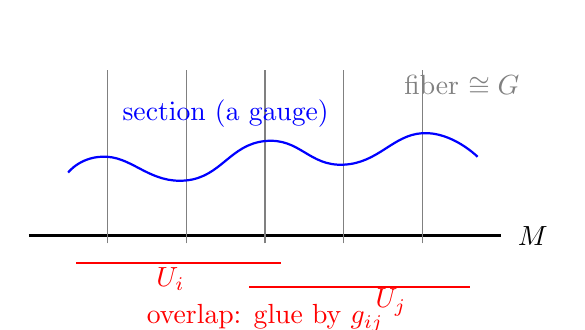
\begin{tikzpicture}[scale=1.0]
  % base line
  \draw[thick] (0,0) -- (6,0);
  \node at (6.4,0) {$M$};
  % fibers
  \foreach \x in {1,2,3,4,5} \draw[gray] (\x,-0.1) -- (\x,2.1);
  \node[gray] at (5.5,1.9) {fiber $\cong G$};
  % section
  \draw[blue,thick] plot[smooth,tension=0.8] coordinates {(0.5,0.8)(1,1.0)(2,0.7)(3,1.2)(4,0.9)(5,1.3)(5.7,1.0)};
  \node[blue] at (2.5,1.55) {section (a gauge)};
  % patches
  \draw[red,thick] (0.6,-0.35) -- (3.2,-0.35);
  \draw[red,thick] (2.8,-0.65) -- (5.6,-0.65);
  \node[red] at (1.8,-0.55) {$U_i$};
  \node[red] at (4.6,-0.85) {$U_j$};
  \node[red] at (3.0,-1.05) {overlap: glue by $g_{ij}$};
\end{tikzpicture}
\end{center}

\begin{eexample}[A small zoo of bundles]
\textbf{(a)} Trivial bundle $P=M\times G$: a global gauge exists; this is the case
implicitly assumed in \S2--\S3. \textbf{(b)} The Hopf bundle
$\Uone\hookrightarrow S^3\to S^2$: the charge-$1$ Dirac monopole. Its transition
function on the $S^2$ equator winds once around $\Uone$. \textbf{(c)} A flat
$G$-bundle: transition functions can be taken \emph{constant}, and the bundle is
classified by a homomorphism $\pi_1(M)\to G$ (we use this constantly for finite $G$ in
\S5). \textbf{(d)} The frame bundle of $M$: structure group $\mathrm{GL}(d)$ (or
$\mathrm{SO}(d)$ with a metric); its connection is the Levi-Civita connection of GR.
\end{eexample}

% ----------------------------------------------------------------------
\subsection{Associated bundles: where matter lives}
\label{sec:associated}
% ----------------------------------------------------------------------

A principal bundle is about the gauge group itself. Matter fields live in
\vocab{associated bundles} built from it, and spelling this out finally explains the
notation $P\times_G V$ used above. Given a representation $(R,V)$ of $G$ (so $V$ is the
vector space the multiplet lives in), form the \vocab{associated vector bundle}
\[
E=P\times_G V\;\defeq\;(P\times V)/\!\sim,\qquad (p\cdot g,\,v)\sim(p,\,R(g)\,v).
\]
In words: take pairs (frame $p$, vector $v$) and declare that rotating the frame by $g$
while rotating the vector by $R(g)$ gives the same physical point. A \vocab{matter field}
in representation $R$ is then a \vocab{section} of $E$: in a local gauge it is an ordinary
$V$-valued function $\psi_i$ on $U_i$, and on overlaps the two descriptions are related by
\[
\psi_i=R(g_{ij})\,\psi_j\qquad\text{on }U_i\cap U_j.
\]
This is the global meaning of the rule ``$\psi\to g\psi$'' from \S3: a gauge
transformation is the transition function $g_{ij}$ acting in the representation $R$. The
covariant derivative $D_\mu\psi$ is the instruction for differentiating such a section in
a way that respects the gluing---which is exactly what the connection provides, next.
Finally, the curvature $F$ will live in the associated bundle for the \emph{adjoint}
representation, the \vocab{adjoint bundle} $\ad P=P\times_G\lie g$; that is what the
phrases ``$F$ transforms in the adjoint'' and ``$F$ is valued in $\ad P$'' mean precisely.

% ----------------------------------------------------------------------
\subsection{Connections: the gauge field as a global object}
% ----------------------------------------------------------------------

What does a connection \emph{do}? It provides \vocab{parallel transport}: a consistent
rule for lifting a path in the base $M$ to a path in the total space $P$, i.e.\ for
carrying an internal frame along as you move through spacetime. Infinitesimally, this is a
choice at each point of $P$ of which directions count as \vocab{horizontal}---the
directions ``along which the frame is not rotating.'' That choice is encoded in a single
$\lie g$-valued $1$-form on $P$.

\begin{ddefinition}[Connection / gauge field]
A \vocab{connection} on $P$ is a $\lie g$-valued $1$-form $\omega\in\Omega^1(P,\lie g)$ on
the total space, subject to two conditions:
\begin{enumerate}[label=(\roman*)]
\item on vertical (along-the-fiber) directions $\omega$ returns the Lie-algebra element
generating them, so the horizontal directions are exactly $\ker\omega$;
\item it is $G$-equivariant, $R_g^*\,\omega=\Ad_{g^{-1}}\omega$ (here $R_g$ is the right
action of $g$ and $R_g^*$ its pullback), so the horizontal directions are carried
consistently around each fiber.
\end{enumerate}
\end{ddefinition}

This is the mathematician's (Ehresmann) definition, and it deliberately looks nothing like
the physicist's $A_\mu$. \emph{The bridge between them is pullback by a section.} Pick a
local gauge, i.e.\ a section $s_i:U_i\to P$. Then
\[
A_i\;\defeq\;s_i^{*}\,\omega\ \in\ \Omega^1(U_i,\lie g)
\]
is an honest $\lie g$-valued $1$-form on the patch $U_i$---and \emph{this is the
physicist's $A_\mu^a T^a\,\dd x^\mu$.} (``Pullback $s_i^*$'' just means: $\omega$ lives on
$P$, the section $s_i$ maps $U_i$ into $P$, and we read $\omega$ back along that map to get
a form on $U_i$.) The abstract $\omega$ is gauge-independent; the familiar $A_\mu$ is what
you see \emph{after} choosing a gauge $s_i$. Two sections over an overlap differ by a
fiber rotation, $s_j=s_i\cdot g_{ij}$, and pulling back $\omega$ along each yields the
\vocab{gluing law}
\[
\boxed{\;A_j=g_{ij}^{-1}A_i\,g_{ij}+i\,g_{ij}^{-1}\dd g_{ij}\;}
\]
This is \emph{identically} the gauge transformation of \S3, now with a sharper meaning: it
is how the one connection $\omega$ looks in two different local gauges. Changing the
section on a single patch, $s_i\to s_i\cdot h(x)$, is an ordinary gauge transformation;
passing between patches is the transition $g_{ij}$; the gluing law shows these are the
\emph{same} operation. That is why ``gauge redundancy'' and ``patching data'' are one
notion, not two.

\begin{eequation}[The definition to carry in your head]
\[
\textbf{A $G$-gauge field on $M$} \;=\; \textbf{a connection on a principal
$G$-bundle over $M$.}
\]
On each patch it is the familiar $A_\mu^a T^a\,\dd x^\mu$; globally it is the patches
\emph{plus} the gluing data $g_{ij}$. Two gauge fields are physically the same iff
related by a (globally defined) gauge transformation, i.e.\ a bundle automorphism.
\end{eequation}

The finite version of parallel transport is the \vocab{holonomy}: lift a loop $\gamma$
horizontally and read off the group element relating the starting frame to the ending one.
In a local gauge this is exactly the path-ordered Wilson line of \S3,
$\Hol(\gamma)=\Pexp\,i\oint_\gamma A$. So the Wilson loop is not an extra gadget bolted
onto gauge theory: it \emph{is} the connection's parallel transport, written in a gauge.

\begin{ddefinition}[Curvature]
The \vocab{curvature} of the connection is the $\lie g$-valued $2$-form
\[
F = \dd A - i\,A\wedge A = \dd A - \tfrac{i}{2}[A,A]
\]
(physics convention, matching \S3; the two forms agree since $A\wedge A=\tfrac12[A,A]$).
Although the local potentials $A_i$ glue by the inhomogeneous law above, the curvature
glues \emph{homogeneously}, $F_j=g_{ij}^{-1}F_i\,g_{ij}$, with no $\dd g$ term. Hence $F$
is a genuinely globally defined $2$-form valued in the adjoint bundle $\ad P$. It obeys the
\vocab{Bianchi identity} $\dd_A F\equiv\dd F-i[A,F]=0$ (for abelian $G$ this is just
$\dd F=0$, the homogeneous Maxwell equations). Geometrically, $F$ measures the failure of
horizontal lifts to close up: the holonomy around an infinitesimal loop in the
$\mu\nu$-plane is $\mathbf 1-iF_{\mu\nu}\,\dd x^\mu\dd x^\nu+\cdots$. This is the precise
sense, promised in \S3.3, in which \emph{curvature is infinitesimal holonomy}.
\end{ddefinition}

\begin{xca}[\textbf{(medium)} the inhomogeneous term cancels in $F$]
Starting from the gluing law for $A$, verify directly that $F=\dd A - iA\wedge A$ glues
covariantly, $F_j = g_{ij}^{-1}F_i g_{ij}$, with no $\dd g$ term. \emph{This is the
calculation that explains why $\tr F^k$ are globally defined and give topological
invariants.}
\end{xca}

% ----------------------------------------------------------------------
\subsection{Topology: characteristic classes, monopoles, instantons}
\label{sec:topology}
% ----------------------------------------------------------------------

Because $\tr F^k$ is globally defined, gauge invariant, and closed (closed by the Bianchi
identity), its integral over a closed cycle does not change under any continuous
deformation of the connection: it is a \vocab{topological invariant} of the bundle. The
systematic recipe for manufacturing such invariants from $F$ is \vocab{Chern--Weil
theory}, and the resulting de Rham classes are the \vocab{characteristic classes}. Two of
them run most of physics.

\begin{eequation}[The two invariants you must know]
\textbf{First Chern number} (abelian flux / monopole charge), over a closed surface
$\Sigma$:
\[
c_1 = \frac{1}{2\pi}\int_\Sigma F \in \ints.
\]
\textbf{Instanton number / second Chern number} (non-abelian, over a closed $4$-manifold
$X$):
\[
k = \frac{1}{8\pi^2}\int_X \tr(F\wedge F) \in \ints.
\]
Integrality is the geometric origin of Dirac charge quantization and of the
quantization of the $\theta$-angle's periodicity.
\end{eequation}

Why are these \emph{integers}, rather than arbitrary real numbers? Both count windings.
For the abelian $c_1$, cover $\Sigma$ by patches; on overlaps the potentials differ by
$\dd\lambda_{ij}$, and applying Stokes patch by patch reduces $\frac{1}{2\pi}\int_\Sigma F$
to the total winding of the transition functions $e^{i\lambda_{ij}}:S^1\to\Uone$ around the
patch boundaries. A map $S^1\to\Uone$ has an integer winding number---this is the
statement $\pi_1(\Uone)=\ints$---so $c_1\in\ints$. This is precisely the monopole
quantization of \S4.1, now recognized as a fact about $\pi_1$ of the gauge group. For the
non-abelian instanton number, a finite-action field on $\reals^4$ must approach pure gauge
at infinity, $A\to i\,g\,\dd g^{-1}$, defining a map $g:S^3_\infty\to G$; its winding lives
in $\pi_3(G)=\ints$ for every simple $G$, and equals $\frac{1}{8\pi^2}\int\tr(F\wedge F)$.
Here $\pi_n(X)$ denotes the $n$-th \vocab{homotopy group}, the set of homotopy classes of
maps $S^n\to X$---the precise bookkeeping of ``how many times one sphere wraps a space.''

\begin{eexample}[Instantons]
On $\reals^4$ with finite action, $A$ must approach pure gauge at infinity,
$A\to ig\,\dd g^{-1}$ with $g:S^3_\infty\to G$. For $G=\mathrm{SU}(2)\cong S^3$ such maps
are classified by $\pi_3(\mathrm{SU}(2))=\ints$, the instanton number $k$ above. An
instanton is a finite-action solution in a fixed topological sector $k\neq0$; it
tunnels between topologically distinct vacua and underlies the $\theta$-vacuum
structure and the resolution of the $\mathrm{U}(1)_A$ problem.
\end{eexample}

\begin{xca}[\textbf{(thinker)} $\theta$-term is topological]
Show that $\frac{\theta}{8\pi^2}\int_X \tr(F\wedge F)$ adds $\theta k$ to the action with
$k\in\ints$, so the path integral $e^{iS}$ is periodic, $\theta\sim\theta+2\pi$. Explain
why this term does not affect the classical equations of motion (it is a total
derivative / depends only on the bundle), yet it has real physical effects
nonperturbatively. \emph{This is your first ``coupling constant that is really a
topological label.''}
\end{xca}

\begin{nnote}[How a practitioner actually uses bundles]
You rarely manipulate $\omega$ on the total space $P$. In practice: (1) work locally
with $A_\mu^a$ as in \S3; (2) remember that globally there may be several patches glued
by $g_{ij}$, which is where topology lives; (3) extract topology from gauge-invariant
integrals $\frac{1}{2\pi}\int F$, $\frac{1}{8\pi^2}\int\tr F^2$, and from holonomies
$\oint A$. The bundle language is the \emph{bookkeeping that guarantees these are
well-defined}; you reach for it precisely when something topological is at stake
(monopoles, instantons, flux sectors, anomalies, finite gauge groups).
\end{nnote}

\begin{ppreview}[Where this is heading]
The phrase ``$A$ is a $\Uone$ gauge field'' now has a precise meaning: $A$ is a
connection on a principal $\Uone$-bundle, equivalently the collection of local
potentials $A_i$ with $\Uone$-valued transition functions, with gauge-invariant content
encoded in holonomies $\oint A$ and Chern numbers $\frac1{2\pi}\int F$. In \S5 we
replace the continuous group by a finite one and discover that ``connection'' still
makes perfect sense---it just becomes an assignment of group elements to paths.
\end{ppreview}

% ======================================================================
\section{Finite-group gauge fields: what is a \texorpdfstring{$\Ztwo$}{Z2}-gauge field?}
\label{sec:finite}
% ======================================================================

Here is the puzzle that sends most students reeling the first time. A finite group like
$\Ztwo$ has \emph{no Lie algebra}: there is no $\lie g$, no $A_\mu^a T^a$, no continuous
$A_\mu(x)$. So what on earth does ``$\mu$ is a $\Ztwo$-gauge field'' mean? The answer is
that we have been overcomplicating ``connection.'' Strip it to its essence.

% ----------------------------------------------------------------------
\subsection{A connection is a rule for parallel transport along paths}
% ----------------------------------------------------------------------

\begin{iintuition}[The essence of a connection]
Forget $A_\mu$. A connection is, at heart, a recipe that assigns to each path
$\gamma:x\to y$ a group element $\Hol(\gamma)\in G$---the holonomy---such that
\textbf{(i)} composing paths multiplies holonomies, $\Hol(\gamma_2\gamma_1) =
\Hol(\gamma_2)\Hol(\gamma_1)$, and \textbf{(ii)} reversing a path inverts it. For a Lie
group this recipe is generated by integrating $A_\mu$ ($\Hol = \Pexp\, i\!\int A$). But
the recipe makes sense for \emph{any} group $G$, including a finite one---we just
specify the group elements directly. \textbf{That is a $G$-gauge field.}
\end{iintuition}

For a finite group there is no continuous local data to integrate; the connection lives
on the discrete skeleton of spacetime. So we put spacetime on a lattice (or a
triangulation / simplicial complex) and assign the data to edges.

% ----------------------------------------------------------------------
\subsection{The lattice definition: link variables}
% ----------------------------------------------------------------------

\begin{ddefinition}[Lattice $G$-gauge field, $G$ any group]
Triangulate (or put a lattice on) spacetime, with vertices, edges, and plaquettes
(2-cells). A \vocab{$G$-gauge field} is an assignment of a group element to each
oriented edge $e$,
\[
g_e \in G, \qquad g_{\bar e} = g_e^{-1},
\]
i.e.\ the holonomy across that link. A \vocab{gauge transformation} is a choice of
group element $h_v\in G$ at each vertex, acting by
\[
g_e \;\longmapsto\; h_{t(e)}\, g_e\, h_{s(e)}^{-1}
\qquad (s,t = \text{source, target of } e).
\]
The \vocab{field strength} (curvature) is the holonomy around each plaquette $p$,
\[
g_p = \prod_{e\in\partial p} g_e \qquad(\text{ordered product around the boundary}),
\]
which transforms by conjugation $g_p\to h\,g_p\,h^{-1}$. The configuration is
\vocab{flat} if $g_p = \mathbf 1$ for every plaquette.
\end{ddefinition}

\begin{center}
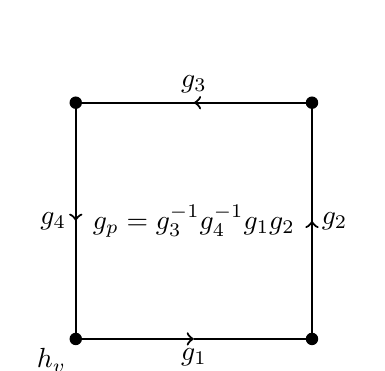
\begin{tikzpicture}[scale=1.5]
  \draw[thick,->] (0,0) -- (1,0); \draw[thick] (1,0)--(2,0);
  \draw[thick,->] (2,0) -- (2,1); \draw[thick] (2,0)--(2,2);
  \draw[thick,->] (2,2) -- (1,2); \draw[thick] (2,2)--(0,2);
  \draw[thick,->] (0,2) -- (0,1); \draw[thick] (0,2)--(0,0);
  \node[below] at (1,0) {$g_1$};
  \node[right] at (2,1) {$g_2$};
  \node[above] at (1,2) {$g_3$};
  \node[left]  at (0,1) {$g_4$};
  \node at (1,1) {$g_p=g_3^{-1}g_4^{-1}g_1 g_2$};
  \foreach \p in {(0,0),(2,0),(2,2),(0,2)} \fill \p circle (1.5pt);
  \node[below left] at (0,0) {$h_v$};
\end{tikzpicture}
\end{center}

\begin{iintuition}[This is literally the continuum story, discretized]
Edge variable $g_e$ $\leftrightarrow$ Wilson line $\Pexp\,i\!\int_e A$ across a link.
Vertex transformation $h_v$ $\leftrightarrow$ gauge function $g(x)$. Plaquette product
$g_p$ $\leftrightarrow$ $\exp(i\!\oint_{\partial p}A) = \exp(iF\cdot\text{area})$, the
infinitesimal-loop holonomy from the Exercise in \S3.3. ``Flat'' $\leftrightarrow$
``$F=0$.'' Nothing new conceptually---we just dropped the requirement that $G$ be
continuous, and the integrals became products.
\end{iintuition}

\begin{eexample}[$\Ztwo$ gauge field, concretely]
\label{ex:z2}
Take $G=\Ztwo=\{+1,-1\}$ (multiplicatively) or $\{0,1\}$ with addition mod $2$. A
$\Ztwo$ gauge field assigns $g_e = \pm1$ to each edge. A gauge transformation flips
$g_e\to h_{t}g_e h_{s}$ with $h_v=\pm1$ at vertices. The plaquette curvature is the
product of the four edge signs around a square; flat means every plaquette product is
$+1$. This is exactly Wegner's $\Ztwo$ lattice gauge theory (a.k.a.\ Ising gauge
theory), and the dynamical version is the deconfined phase that is the toric
code.\footnote{Lattice gauge theory of finite groups: Kogut, \emph{Rev.\ Mod.\ Phys.}
\textbf{51} (1979). For the $\Ztwo$/toric-code/condensed-matter side of everything in
this section, McGreevy, \emph{Generalized Symmetries in Condensed Matter},
\texttt{arXiv:2204.03045}; and Harlow, \emph{8.325 (QFT III)}~\S8.1 for a clean
Hamiltonian lattice answer to ``what is a gauge field?''} When
someone writes ``$\mu$ is a $\Ztwo$-gauge field,'' $\mu$ is precisely this edge
assignment (often written additively, $\mu\in C^1(M;\Ztwo)$; see below).
\end{eexample}

\begin{xca}[\textbf{(easy)} counting $\Ztwo$ configurations]
On a single square (4 edges, 4 vertices, 1 plaquette), count: (a) the number of
$\Ztwo$ gauge field configurations; (b) the number of gauge transformations; (c) the
number of \emph{flat} configurations up to gauge. \emph{Hint for (c): you should find
that on the disk every flat connection is gauge-trivial.}
\end{xca}

% ----------------------------------------------------------------------
\subsection{The cohomological repackaging (why people say ``cocycle'')}
% ----------------------------------------------------------------------

For an abelian finite group like $\ZN$, write the group additively. Then a gauge field
is a function $a$ from edges to $\ZN$: a \vocab{$1$-cochain}, $a\in C^1(M;\ZN)$. The
plaquette curvature is $(\dd a)_p = \sum_{e\in\partial p} a_e$, the \vocab{coboundary}.
A gauge transformation shifts $a$ by $\dd\lambda$ for a $0$-cochain $\lambda$ (the
vertex data). So the picture is a perfect discrete analogue of $A\to A+\dd\lambda$,
$F=\dd A$:

\begin{eequation}[Continuum vs.\ finite, side by side]
\[
\begin{array}{c|c|c}
 & \text{continuous } \Uone & \text{finite } \ZN \\\hline
\text{gauge field} & A\in \Omega^1(M) & a\in C^1(M;\ZN)\\
\text{gauge transf.} & A\to A+\dd\lambda & a\to a+\dd\lambda\\
\text{field strength} & F=\dd A & \dd a\\
\text{flat} & \dd A=0 & \dd a=0\\
\text{flat mod gauge} & H^1(M;\reals)/\ints \!\cong\! \mathrm{Hom}(\pi_1,\Uone) & H^1(M;\ZN)\cong\mathrm{Hom}(\pi_1,\ZN)
\end{array}
\]
\end{eequation}

\begin{ddefinition}[Flat finite gauge field = cohomology class = representation of $\pi_1$]
A \vocab{flat} $G$-gauge field ($g_p=\mathbf 1$ for all $p$) up to gauge equivalence is
the same data as a homomorphism $\rho:\pi_1(M)\to G$ up to conjugation. For abelian $G$
this is $H^1(M;G)=\mathrm{Hom}(\pi_1(M),G)$. In words: \emph{a flat finite gauge field
is completely determined by the group elements you pick up going around the
non-contractible loops of spacetime.}
\end{ddefinition}

\begin{iintuition}[Finite gauge fields are pure holonomy]
For a continuous group, $A$ has local wiggles (curvature) \emph{and} global holonomies.
For a finite group there is no local wiggle room---the natural configurations are flat,
and \emph{all} the information is the holonomy around non-contractible cycles. This is
why finite gauge fields are intrinsically topological objects, and why $\Ztwo$ gauge
fields show up everywhere topology matters (spin structures, SPT phases, discrete
$\theta$-angles, symmetry defects).
\end{iintuition}

\begin{eexample}[A flat $\Ztwo$ field on a circle / torus]
On $S^1$: $\pi_1=\ints$, so $\mathrm{Hom}(\ints,\Ztwo)=\Ztwo$. There are exactly two
flat $\Ztwo$ gauge fields up to gauge: ``trivial'' (holonomy $+1$ around the circle) and
``nontrivial'' (holonomy $-1$). On the torus $T^2$: $\pi_1=\ints^2$, so there are
$2\times2=4$ classes, labelled by the holonomies around the two cycles. \emph{These four
sectors are exactly the four spin structures on the torus, and the four ``twisted
boundary condition'' sectors you sum over when gauging a $\Ztwo$ symmetry (\S7).}
\end{eexample}

\begin{eexample}[Spin structures and $(-1)^F$: a $\Ztwo$ gauge field you have used]
A choice of periodic vs.\ antiperiodic boundary conditions for a fermion around a cycle
\emph{is} a flat $\Ztwo$ background for fermion parity $(-1)^F$. The ``$-$'' in the NS
sector, the Matsubara antiperiodicity of thermal fermions, the spin structure on a
Riemann surface---these are all the statement ``turn on a nontrivial $\Ztwo$ gauge
field.'' You have been using $\Ztwo$ gauge fields since your first thermal field theory
computation without calling them that.
\end{eexample}

\begin{xca}[\textbf{(classic)} flat $\ZN$ fields on surfaces]
Compute the number of gauge-inequivalent flat $\ZN$ gauge fields on (a) the sphere
$S^2$, (b) the torus $T^2$, (c) a genus-$h$ surface $\Sigma_h$. \emph{Answers in terms
of $N$ and $h$; relate to $H^1(\Sigma_h;\ZN)$.}
\end{xca}

\begin{xca}[\textbf{(thinker)} discrete Wilson lines and non-abelian holonomy]
For $G=S_3$ (non-abelian), explain why ``flat connections up to gauge'' is
$\mathrm{Hom}(\pi_1,S_3)/\text{conjugation}$ rather than $H^1$. On $T^2$, this means
pairs of commuting elements $(a,b)$ up to simultaneous conjugation. Enumerate them.
\emph{This is the configuration sum for finite \emph{non-abelian} gauge theory
(Dijkgraaf--Witten).}\footnote{Dijkgraaf \& Witten, \emph{Topological gauge theories and
group cohomology}, \emph{Comm.\ Math.\ Phys.} \textbf{129} (1990)---finite gauge theory
and the origin of the discrete theta term as a class in $H^d(BG;\Uone)$.}
\end{xca}

\begin{nnote}[``$\mu$ is a $\Ztwo$ gauge field'' --- decoded]
When a paper introduces ``a $\Ztwo$ gauge field $\mu$,'' it means: a $\Ztwo$-valued
$1$-cochain (assignment of $\pm1$ to links / a class in $H^1$), defined up to
$\mu\to\mu+\dd\lambda$. If $\mu$ is \emph{background}, it is a fixed choice probing a
$\Ztwo$ symmetry (twisted boundary conditions / a network of $\Ztwo$ symmetry defects,
\S6). If $\mu$ is \emph{dynamical}, you sum over all its classes (\S7); that is
$\Ztwo$ gauge theory. The same symbol, two completely different roles---which is exactly
the background-vs-dynamical distinction we turn to now.
\end{nnote}

% ======================================================================
\section{Background gauge fields: probing a global symmetry}
% ======================================================================

We now reach the conceptual heart of the modern point of view. We have two kinds of
gauge field, distinguished not by their geometry (both are connections) but by their
\emph{role in the path integral}.

% ----------------------------------------------------------------------
\subsection{Coupling a global symmetry to a background}
% ----------------------------------------------------------------------

Suppose a theory has a global symmetry $G$ with Noether current $j^\mu$ (continuous
case) or symmetry operators $U_g$ (general case). The defining move of the modern
viewpoint:

\begin{ddefinition}[Background gauge field]
To \vocab{couple the symmetry $G$ to a background gauge field} is to introduce a
\emph{fixed, non-dynamical} $G$-connection $A$ on spacetime and deform the theory so
that the global symmetry is promoted to a local one \emph{with $A$ transforming as a
connection}, but \textbf{without integrating over $A$}. The partition function becomes a
functional of the background,
\[
Z[A] = \int \mathcal{D}(\text{fields})\; e^{iS[\text{fields};\,A]},
\]
and we keep $A$ as an external knob. Concretely, for a continuous symmetry one adds
$\int A_\mu j^\mu + \mathcal O(A^2)$ (minimal coupling); for a finite symmetry one
inserts a network of symmetry defects (\S6.3).
\end{ddefinition}

\begin{iintuition}[A background field is a knob, a source, a probe]
Setting $A=0$ recovers the original theory. Turning on $A\neq 0$ lets you ask: how does
the theory respond to a position-dependent symmetry transformation? It is the same idea
as turning on a background electromagnetic field to probe a material, or an external
metric $g_{\mu\nu}$ to probe the stress tensor. You are \emph{not} adding new dynamical
degrees of freedom; you are interrogating the ones you have. The current $j^\mu$ is the
linear response: $\langle j^\mu(x)\rangle = -i\,\delta \log Z[A]/\delta A_\mu(x)$.
\end{iintuition}

\begin{eexample}[The simplest background gauge field: a particle on a ring]
Nothing illustrates ``background field $=$ knob'' better than a free particle of unit
charge on a circle of circumference $2\pi$, threaded by Aharonov--Bohm flux $\theta$.
The flux is a flat background $\Uone$ gauge field $A=\frac{\theta}{2\pi}\dd x$: locally
pure gauge ($F=0$), but with physical holonomy $\oint A=\theta$. Minimal coupling shifts
the momentum, giving the spectrum
\[
E_n = \tfrac12\Big(n-\tfrac{\theta}{2\pi}\Big)^2,\qquad n\in\ints .
\]
Three lessons in one formula: (i) the spectrum depends \emph{only} on the holonomy
$\theta$, not on the pointwise $A$---the background's physical content is its holonomy;
(ii) $\theta\sim\theta+2\pi$ (relabel $n$), so the knob is $\Uone$-valued, as a flat
$\Uone$ background should be; (iii) at $\theta=\pi$ two levels cross---the first hint of
the kind of degeneracy that a mixed 't Hooft anomaly at $\theta=\pi$ enforces (\S8). This
toy model is the entire idea of $Z[A]$ stripped to one degree of freedom.\footnote{This
particle-on-a-ring / $\theta$-angle picture, and the $\theta=\pi$ level crossing, are
developed in Tong, \emph{Lectures on Gauge Theory}~\S1.2,~\S2.2.3.}
\end{eexample}

\begin{eequation}[Currents and Ward identities for free]
Differentiating $Z[A]$ in the background generates correlators of the current:
\[
\langle j^{\mu_1}(x_1)\cdots j^{\mu_n}(x_n)\rangle
= \frac{(-i)^n}{Z}\frac{\delta^n Z[A]}{\delta A_{\mu_1}(x_1)\cdots \delta A_{\mu_n}(x_n)}\bigg|_{A=0}.
\]
\textbf{Background gauge invariance of $Z[A]$ is the statement that $j^\mu$ is
conserved}---the Ward identities are just $Z[A^\lambda]=Z[A]$ expanded in $\lambda$.
\end{eequation}

% ----------------------------------------------------------------------
\subsection{The defining property: background gauge invariance}
% ----------------------------------------------------------------------

\begin{ddefinition}[Having a symmetry, modern definition]
A theory \vocab{has} the global symmetry $G$ (non-anomalously) if its partition
function in a background can be made \emph{invariant} under background gauge
transformations,
\[
Z[A^\lambda] = Z[A]\qquad\text{for all }\lambda:M\to G,
\]
possibly after adding local counterterms built from $A$. If no choice of local
counterterms achieves this---if $Z[A^\lambda]=Z[A]\,e^{i\int \omega(\lambda,A)}$ with a
phase that cannot be removed---the symmetry has a \vocab{'t Hooft anomaly} (\S8).
\end{ddefinition}

\begin{iintuition}[Why phrase symmetry this way?]
This definition is robust in ways the Noetherian ``there is a conserved current''
definition is not. It (1) works for finite symmetries with no current; (2) makes
anomalies visible as a sharp obstruction (a residual phase); (3) is manifestly
RG-invariant---if you can couple to a background in the UV you can in the IR, which is
the engine of 't Hooft anomaly matching; (4) generalizes verbatim to higher-form
symmetries by letting $A$ be a higher-form background. This is why ``couple to a
background and study $Z[A]$'' \emph{is} the modern definition of a symmetry.
\end{iintuition}

\begin{eexample}[Free Dirac fermion in a background $\Uone$]
Take a free massless Dirac fermion in $4$d with its vector $\Uone_V$ symmetry. Coupling
to a background $A_\mu$ via $\sl{D} = \gamma^\mu(\partial_\mu - iA_\mu)$ gives
$Z[A]$. The vector current is conserved for all $A$: $Z[A]$ is $\Uone_V$
background-gauge-invariant. But the \emph{axial} current $j_5^\mu$ is \emph{not}: under
an axial background gauge transformation $Z$ picks up the famous phase
$\propto \int \lambda\, F\wedge F$. That is the chiral (ABJ) anomaly, our first example
of an 't Hooft anomaly, and it is why $\pi^0\to\gamma\gamma$.
\end{eexample}

\begin{iintuition}[Why the chiral anomaly is unavoidable: spectral flow]
You can \emph{see} the chiral anomaly without a single Feynman diagram. Put a $2$d
massless Dirac fermion in a box and fill the Dirac sea; left-movers and right-movers have
separate Fermi seas. Now adiabatically turn on a background electric field
$E=\partial_t A_x$ (a time-dependent holonomy of $A$). Each single-particle level's
momentum shifts as $\dot p = E$, so states flow \emph{up} through the right-moving sea
and \emph{down} through the left-moving sea: the number of right-movers and left-movers
each change, even though total charge is conserved. The axial charge
$Q_5=N_R-N_L$ is therefore \emph{not} conserved, at a rate fixed purely by how many
levels crossed---i.e.\ by $\int E$. That counting is rigid (an integer flow), which is
exactly why the anomaly coefficient cannot be tuned away by any local counterterm.\footnote{The
spectral-flow / level-crossing derivation is in Tong, \emph{Lectures on Gauge
Theory}~\S3.1; the relation to the Atiyah--Singer index and instanton zero modes is
\S3.3.} This is the microscopic face of ``the anomaly is a quantized obstruction.''
\end{iintuition}

\begin{eexample}[Background metric is a background gauge field for spacetime symmetry]
The stress tensor $T^{\mu\nu}$ is the current for translations; coupling it to a
background means putting the theory on a curved metric $g_{\mu\nu}$, giving $Z[g]$.
``Background diffeomorphism + Weyl invariance of $Z[g]$'' is exactly the statement of no
gravitational/conformal anomaly; the failure is the trace anomaly
$\langle T^\mu_\mu\rangle\sim c\,(\text{curvature})$. \emph{Same machine, symmetry
$=$ spacetime symmetry, background $=$ metric.} Keep this analogy close: it tells you
the metric is ``just'' the background gauge field for the Poincar\'e/conformal symmetry.
\end{eexample}

\begin{xca}[\textbf{(medium)} current as response, explicitly]
For the complex scalar of \S2 coupled to background $A_\mu$, compute
$\delta \log Z[A]/\delta A_\mu$ at $A=0$ and check it equals $\langle j^\mu\rangle$ with
$j^\mu = i(\phi^*\partial^\mu\phi - \phi\,\partial^\mu\phi^*)$. Then show invariance of
$Z[A]$ under $A\to A+\dd\lambda$ at linear order reproduces $\partial_\mu j^\mu=0$.
\end{xca}

% ----------------------------------------------------------------------
\subsection{Backgrounds for finite symmetries: defect networks}
% ----------------------------------------------------------------------

For a finite symmetry $G$ there is no current to write $\int A_\mu j^\mu$. Instead,
turning on a background $a\in H^1(M;G)$ means \emph{inserting a network of symmetry
defects} Poincar\'e-dual to $a$.

\begin{iintuition}[Background $=$ symmetry-defect network $=$ twisted boundary conditions]
A $G$ symmetry operator $U_g$ is supported on a codimension-$1$ surface; crossing it
acts on operators by $g$ (\S9). A background $a$ specifies, for each codimension-$1$
sheet in a chosen dual cell decomposition, which $U_g$ sits there. On a spacetime cycle,
this is exactly a \vocab{twisted boundary condition}: ``identify fields up to the action
of $g$ when you go around.'' For $\Ztwo$ on a circle, $a=$ nontrivial means
antiperiodic/twisted; $Z[a]$ is the twisted partition function $\tr\big(g\,e^{-\beta
H}\big)$.
\end{iintuition}

\begin{eexample}[Twisted partition functions of the Ising model]
The $2$d Ising CFT has a $\Ztwo$ spin-flip symmetry. Its torus partition functions in
the four $\Ztwo$ backgrounds $a\in H^1(T^2;\Ztwo)=(\Ztwo)^2$ are the four sectors
$Z[a] = \tr_{\mathcal H_b}(g^{a_t}\,e^{-\beta H})$ with periodic/twisted space
($a_s$) and time ($a_t$) directions. Modular transformations permute these four
$Z[a]$'s; demanding consistency under gauging $\Ztwo$ (summing them, \S7) reproduces
Kramers--Wannier duality. \emph{This little $2\times2$ table of twisted partition
functions is the entire input to a huge amount of modern $2$d physics.}
\end{eexample}

% ----------------------------------------------------------------------
\subsection{Background vs.\ dynamical: the clean contrast}
% ----------------------------------------------------------------------

\begin{center}
\renewcommand{\arraystretch}{1.35}
\begin{tabular}{p{0.235\textwidth}|p{0.33\textwidth}|p{0.33\textwidth}}
 & \textbf{Background gauge field} & \textbf{Dynamical gauge field}\\\hline
Role in path integral & fixed external data; \emph{not} integrated over & a field; \emph{integrated} over ($\int\mathcal D A$ or $\sum_a$)\\
Associated symmetry & a \emph{global} symmetry it probes & gauge ``symmetry'' is a \emph{redundancy}, not a symmetry\\
Equations of motion & none (it is a source) & has its own EOM / Gauss-law constraint\\
What you compute & $Z[A]$ as a functional; correlators of $j$ & a new theory's $Z$; gauge-invariant operators only\\
Gauge transformations & a true symmetry of $Z[A]$ (or anomalous) & a redundancy you quotient by\\
Examples & external EM field, curved metric, $\Ztwo$ twist $\mu$ & photon in QED, gluon, $\Ztwo$ gauge theory\\
\end{tabular}
\end{center}

\begin{nnote}[The slogan]
\textbf{Background: you fix it and study the response. Dynamical: you sum over it and
get a new theory.} The very same connection $A$ can be either, depending on whether it
appears under the path-integral measure. ``Gauging'' is the operation that turns the
first into the second.
\end{nnote}

\begin{xca}[\textbf{(easy)} which is which?]
Classify each as background or dynamical, and name the (global or gauge) group:
(a) the photon in QED; (b) the external magnetic field in the quantum Hall effect;
(c) the gluon field; (d) the metric in a non-gravitational QFT; (e) the $\Ztwo$ field
recording fermion boundary conditions; (f) the $\Ztwo$ field in the toric code.
\end{xca}

% ======================================================================
\section{Gauging: making a symmetry local}
% ======================================================================

\begin{ddefinition}[Gauging]
To \vocab{gauge} a global symmetry $G$ is to promote its background gauge field from
fixed to dynamical: sum/integrate over $A$ in the path integral. Schematically,
\[
Z_{\text{gauged}} = \int \mathcal D A \; Z[A]
\quad(\text{continuous}),
\qquad
Z_{\text{gauged}}[M] = \frac{1}{|G|^{\,N_0}}\sum_{\{g_e\}} Z[\{g_e\}]
\quad(\text{finite}).
\]
For continuous $G$ one also adds a dynamical kinetic term $\frac1{2g^2}\int\tr F^2$. For
finite $G$ the sum runs over \emph{all} link configurations $\{g_e\}$ and is divided by
the number of gauge transformations $|G|^{N_0}$ ($N_0=$ number of vertices)---the volume
of the gauge group, i.e.\ exactly one factor of $1/|G|$ per redundancy. Restricted to
\emph{flat} fields this collapses to a sum over $\mathrm{Hom}(\pi_1(M),G)/\text{conj.}$
(equivalently $H^1(M;G)$ for abelian $G$, the configurations of \S5). The result is a
\emph{new theory} in which $G$ is a redundancy.\footnote{Precise lattice prescription
(and its higher-form version): Kapustin--Seiberg \texttt{1401.0740}~\S8. Equivalently
one writes the gauged partition function as a weighted sum over twisted sectors
$Z_{\text{gauged}}=\sum_a h_a\,Z_a$ (GKSW \texttt{1412.5148}, eq.~2.5); the freedom in
the weights $h_a$ is the discrete theta angle / discrete torsion of the next exercise.}
\end{ddefinition}

\begin{iintuition}[Gauging in one breath]
``Gauging'' literally means ``declaring the symmetry to be a local redundancy of
description rather than a physical operation.'' Operationally you do this by making its
gauge field dynamical. Before: $A$ is a knob, the symmetry acts on states. After: $A$
fluctuates, only $G$-invariant data is physical, and the symmetry no longer maps
distinct physical states to one another---it relates descriptions of the \emph{same}
state. You can only do this if there is no 't Hooft anomaly (\S8): an anomaly is exactly
the obstruction to making $Z[A]$ invariant, hence to summing over $A$ consistently.
\end{iintuition}

% ----------------------------------------------------------------------
\subsection{What gauging produces: new operators, new symmetries}
% ----------------------------------------------------------------------

Gauging changes the operator content in two systematic ways:
\begin{itemize}
\item \textbf{Projection.} Only $G$-invariant (gauge-invariant) operators survive.
Charged local operators are projected out (or must be attached to Wilson lines).
\item \textbf{New extended operators.} Wilson lines $\tr\,\Pexp\,i\!\oint A$ and (for
$\theta$-like data) 't Hooft/vortex operators appear, charged under \emph{new} symmetries
that did not exist before gauging---the \vocab{quantum} or \vocab{dual} symmetry. For
gauging a finite abelian $G$ in $d$ dimensions you generate a dual
$\widehat G=\mathrm{Hom}(G,\Uone)$ symmetry that is a $(d-2)$-form symmetry (\S9).
\end{itemize}

\begin{eexample}[Gauging $\Uone$: scalar QED, and a dual current]
Gauging the global $\Uone$ of the complex scalar (\S2) by making $A_\mu$ dynamical gives
scalar QED. The would-be charged operator $\phi$ is no longer gauge invariant on its
own. In $3$d a new $\Uone_{\text{top}}$ ``topological'' symmetry appears with current
$j^\mu_{\text{top}}=\frac1{2\pi}\epsilon^{\mu\nu\rho}\partial_\nu A_\rho$, whose charge
is the magnetic flux; in $4$d the analogous structure is the magnetic $1$-form symmetry
with current $\star F$. \emph{Gauging gives with one hand (a dual symmetry) what it takes
with the other (the original charged operators).}
\end{eexample}

\begin{eexample}[Gauging $\Ztwo$ in $2$d: orbifolds and Kramers--Wannier]
\label{ex:KW}
Gauge the $\Ztwo$ symmetry of the $2$d Ising model by summing $Z[a]$ over the four
backgrounds $a\in H^1(T^2;\Ztwo)$ with the right normalization. The result is again an
Ising model---but with a \emph{dual} $\widehat\Ztwo$ symmetry exchanged with the
original. This is Kramers--Wannier duality realized as ``gauging a $\Ztwo$.'' In string
theory the very same sum over $Z[a]$ is an \vocab{orbifold}. Gauging a finite symmetry =
orbifolding; the dual symmetry $\widehat\Ztwo$ is the ``quantum symmetry'' of the
orbifold. \emph{This single example---gauge $\Ztwo$, get dual $\Ztwo$, recover a
duality---is the prototype for an enormous amount of modern QFT.}
\end{eexample}

\begin{xca}[\textbf{(medium)} gauging twice returns home]
Argue that gauging a finite abelian $G$ produces a theory with dual symmetry
$\widehat G$, and that gauging $\widehat G$ in turn recovers the original theory. (In
$2$d, $\widehat G\cong G$, so ``gauge $\Ztwo$ twice $=$ identity.'') \emph{This is the
abstract content of Kramers--Wannier self-duality.}
\end{xca}

\begin{xca}[\textbf{(thinker)} discrete theta angle / choice of gauging]
When you gauge $G$ you may add a phase weight to each background: a \vocab{discrete
theta angle} valued in $H^d(BG;\Uone)$ ($\sim$ a Dijkgraaf--Witten term). For
$G=\Ztwo$ in $2$d, $H^2(B\Ztwo;\Uone)=0$, but in $3$d, $H^3(B\Ztwo;\Uone)=\Ztwo$ gives
\emph{two} inequivalent ways to gauge. Explain why ``how you gauge'' is extra data, not
canonical, and connect it to stacking with an SPT before gauging.
\end{xca}

% ----------------------------------------------------------------------
\subsection{Gauging a spacetime symmetry; subtleties}
% ----------------------------------------------------------------------

\begin{eexample}[Gauging gives gravity / orientifolds / time-reversal subtleties]
Gauging translations \& rotations (making the metric dynamical) gives gravity. Gauging
a $\Ztwo$ reflection or time-reversal gives unoriented/pin geometries (orientifolds).
These cases carry extra subtleties (you must sum over geometries, spin structures,
orientations), but the logic is identical: take a background (the metric, the
orientation), make it dynamical.
\end{eexample}

\begin{nnote}[Gauging is not free: the anomaly gate]
You cannot gauge a symmetry with an 't Hooft anomaly: the sum $\sum_a Z[a]$ (or
$\int\mathcal D A\,Z[A]$) is not well defined / not gauge invariant precisely because
$Z[A^\lambda]\neq Z[A]$. The anomaly is the gate that decides whether gauging is even
possible. That is why anomalies, which sound like a technical pathology, are actually
the central organizing constraint of the modern program---next section.
\end{nnote}

% ======================================================================
\section{'t Hooft anomalies and anomaly inflow}
% ======================================================================

% ----------------------------------------------------------------------
\subsection{Definition and the meaning of the phase}
% ----------------------------------------------------------------------

\begin{ddefinition}['t Hooft anomaly]
A global symmetry $G$ has an \vocab{'t Hooft anomaly} if, after coupling to a background
$A$, the partition function cannot be made background-gauge-invariant by any local
counterterm; instead
\[
Z[A^\lambda] = Z[A]\,\exp\!\Big(i\!\int_{M_d}\!\alpha(\lambda,A)\Big),
\]
with a definite, counterterm-independent phase $\alpha$. Crucially, $Z[A]$ is still
well defined and the symmetry still acts on the Hilbert space (this is \emph{not} the
inconsistency of a gauged anomaly); what fails is only background gauge invariance.
\end{ddefinition}

\begin{iintuition}[Anomaly = an obstruction you cannot localize away]
A would-be symmetry violated by a local, removable term is no anomaly---just a bad
regulator. An 't Hooft anomaly is a violation that no local counterterm can absorb. The
sharp test: can you write $Z[A]$ as the boundary value of a \emph{local} $(d{+}1)$-dim
functional and restore invariance? If not, the leftover is the anomaly. This obstruction
is quantized (it lives in a discrete classification), hence rigid: it cannot drift under
continuous deformations, which is what makes it RG-invariant.
\end{iintuition}

% ----------------------------------------------------------------------
\subsection{Anomaly inflow: the bulk SPT}
% ----------------------------------------------------------------------

\begin{eequation}[The inflow picture]
An anomalous $d$-dimensional theory is the boundary of a $(d{+}1)$-dimensional
\vocab{invertible}/SPT theory:
\[
Z_{d}[A] \;=\; (\text{boundary of})\;\exp\!\Big(i\!\int_{X_{d+1}}\!\omega(A)\Big),
\qquad \partial X_{d+1}=M_d.
\]
The bulk term $\omega(A)$ is gauge invariant in the closed bulk; its variation localizes
to the boundary and produces exactly the anomalous phase $\alpha$. The anomaly is
\emph{classified} by which bulk SPT you need: an element of group cohomology
$H^{d+1}(BG;\Uone)$ (or, more completely, of a cobordism group
$\Omega^{d+1}_G$).\footnote{Anomalies as boundary modes of invertible/SPT phases, and
their cobordism classification, are developed in Tachikawa's TASI~2019 lectures
\emph{Anomalies and topological phases} and his \emph{Lectures on topological phases for
mathematicians}.}
\end{eequation}

\begin{eexample}[The $2$d chiral fermion's anomaly inflow]
A single right-moving complex fermion in $2$d has a $\Uone$ anomaly; it lives on the
boundary of a $3$d $\Uone$ Chern--Simons term $\frac{k}{4\pi}\int A\,\dd A$. The
non-invariance of $\mathrm{CS}$ on a manifold with boundary is precisely the $2$d
anomalous phase. This is the field-theoretic skeleton of the integer quantum Hall edge:
a $(2{+}1)$d bulk with a chiral edge that cannot exist on its own.
\end{eexample}

\begin{eexample}[Mixed anomaly: momentum vs.\ winding of the $2$d compact boson]
The free compact boson $\phi\sim\phi+2\pi$ in $2$d has two $\Uone$ symmetries: a
\vocab{momentum} symmetry ($\phi\to\phi+c$, current $\propto\star\dd\phi$) and a
\vocab{winding} symmetry (current $\frac{1}{2\pi}\dd\phi$, charge $=$ winding number).
Couple backgrounds $A_m,A_w$ for both. No local counterterm makes $Z[A_m,A_w]$ invariant
under both at once; the leftover is a \vocab{mixed anomaly} with bulk inflow
\[
\textstyle Z[A_m^{\lambda},A_w] = Z[A_m,A_w]\,
\exp\!\big(\tfrac{i}{2\pi}\!\int_{M_2}\lambda\,\dd A_w\big),
\qquad \text{$3$d SPT}\ \ \tfrac{1}{2\pi}\!\int_{X_3} A_m\wedge \dd A_w .
\]
(Note the bulk term is a genuine $3$-form integrated over a $3$-manifold---contrast a
mass-dimension slip like ``$\int_{X_3} a_1\cup a_2$,'' which is only a $2$-form.)
\textbf{Consequence:} you cannot gauge momentum and winding simultaneously. Gauging the
momentum $\Uone$ \emph{is} T-duality, which exchanges the two symmetries (and inverts the
radius); the anomaly is precisely why the theory cannot be trivially gapped while
preserving both---consistent with the free boson being a CFT. \emph{This is the cleanest
mixed anomaly in physics, and it secretly powers a duality you already know.}
\end{eexample}

% ----------------------------------------------------------------------
\subsection{'t Hooft anomaly matching: the payoff}
% ----------------------------------------------------------------------

\begin{ttheorem}['t Hooft anomaly matching]
Because the anomaly is a discrete, deformation-invariant obstruction, it is the
\emph{same} in the UV and the IR of any RG flow. Therefore whatever degrees of freedom
the theory flows to must reproduce the UV anomaly. In particular, a nonzero anomaly
forbids a trivially gapped symmetric vacuum: the IR must contain massless particles, or
spontaneously break the symmetry, or be a nontrivial TQFT.
\end{ttheorem}

\begin{iintuition}[Why this is the workhorse of hep-th]
Anomaly matching is one of the very few \emph{exact, nonperturbative} constraints we
have on strongly-coupled QFT.\footnote{The matching principle originates in 't Hooft's
1980 Carg\`ese lecture \emph{Naturalness, chiral symmetry, and spontaneous chiral
symmetry breaking}.} 't Hooft's original use: the anomalies of QCD's chiral
$\mathrm{SU}(N_f)\times\mathrm{SU}(N_f)$ symmetry, computed on free quarks in the UV,
must be matched in the confined IR---either by massless baryons (hard) or by chiral
symmetry breaking with Goldstones (what nature does). Modern uses: ruling out trivial
gapped phases, deriving the existence of edge modes, constraining the IR of
$\theta=\pi$ gauge theories (Gaiotto--Kapustin--Komargodski--Seiberg), and constructing
deconfined criticality.\footnote{The $\theta=\pi$ mixed anomaly between time-reversal and
the center one-form symmetry, and its IR consequences, are worked out in
Gaiotto--Kapustin--Komargodski--Seiberg, \emph{Theta, Time-Reversal, and Temperature},
\texttt{arXiv:1703.00501}---the template for end-of-chapter Exercise~10.6.} This is
precisely the ``Seiberg-style'' reasoning you are heading toward.
\end{iintuition}

\begin{xca}[\textbf{(classic)} anomaly forbids a trivial gap]
Suppose a theory has a $G$ symmetry with a nonzero 't Hooft anomaly. Argue that it
\emph{cannot} have a unique, symmetric, gapped ground state on every spatial manifold.
\emph{Hint: a trivially gapped symmetric phase has $Z[A]\to$ a manifestly invariant
local counterterm in the deep IR, contradicting the anomalous phase.}
\end{xca}

\begin{xca}[\textbf{(thinker)} anomaly vs.\ gauging, made precise]
Explain, using $Z[A^\lambda]=Z[A]e^{i\int\alpha}$, why an 't Hooft anomaly is exactly
the obstruction to gauging $G$. Then explain why a \emph{mixed} anomaly between $G_1$
and $G_2$ still allows gauging $G_1$ \emph{alone}, but at the cost of the dual symmetry
inheriting an anomaly / $G_2$ becoming anomalous or extended. \emph{This is the
``anomaly is conserved under gauging'' principle.}
\end{xca}

% ======================================================================
\section{The modern point of view, and a preview of generalized symmetries}
\label{sec:higherform}
% ======================================================================

We can now assemble the pieces into the picture that organizes contemporary hep-th.

\begin{eequation}[The modern point of view, in one box]
A QFT is characterized by its \textbf{symmetries}; a symmetry is characterized by how it
\textbf{couples to background gauge fields}, i.e.\ by the functional $Z[A]$ together with
its (possibly anomalous) transformation $Z[A^\lambda]=Z[A]e^{i\int\alpha}$. From this
data one reads off conserved currents (derivatives of $Z$), selection rules (Ward
identities), 't Hooft anomalies (the phase $\alpha$, classified by a bulk SPT), and the
possible \textbf{gaugings} (sum over $A$, allowed iff $\alpha=0$ for that subgroup),
which generate \textbf{dualities} and \textbf{new (dual) symmetries}. Everything is
phrased in the language of backgrounds and defects rather than Lagrangians.
\end{eequation}

% ----------------------------------------------------------------------
\subsection{Symmetries as topological operators}
% ----------------------------------------------------------------------

\begin{iidea}[The Gaiotto--Kapustin--Seiberg--Willett reframing]
A global symmetry is a \vocab{topological operator}. For an ordinary ($0$-form)
symmetry $G$, the operator $U_g(\Sigma_{d-1})$ lives on a codimension-$1$ surface
$\Sigma$, and ``acting with the symmetry'' is sweeping $U_g$ across space. Topological
means correlators are unchanged under continuous deformations of $\Sigma$ that don't
cross charged insertions---which is just current conservation $\dd\star j=0$ restated.
A charged local operator $\op(x)$ is detected because moving $U_g$ \emph{through} $x$
multiplies $\op$ by its charge: the symmetry operator and the charged operator
\vocab{link}. Background gauge field $A$ $=$ an inserted network of these $U_g$'s.
\end{iidea}

\begin{reemark}[The unification: transition functions \emph{are} the defect network]
This closes a loop opened in \S4. There, a $G$-bundle was specified by patches glued
with transition functions $g_{ij}$ on overlaps (satisfying the cocycle condition on
triple overlaps). Here, a background flat connection is a network of defects $U_g$ on
codimension-$1$ sheets, joined at junctions (satisfying a consistency condition where
sheets meet). \emph{These are the same data:} put a defect $U_{g_{ij}}$ on the wall dual
to each overlap $U_i\cap U_j$, and the cocycle condition $g_{ij}g_{jk}=g_{ik}$ becomes
the requirement that the defects fuse consistently at the triple-overlap junction. So
``$\Ztwo$ gauge field'' (\S5), ``transition functions of a bundle'' (\S4), and ``network
of $\Ztwo$ symmetry defects'' (\S6.3) are three names for one object. An 't Hooft anomaly
is then the statement that no consistent set of junction phases exists.\footnote{This
defect/transition-function dictionary, and anomalies as missing topological junctions,
are GKSW \texttt{1412.5148}~\S2.}
\end{reemark}

\begin{iintuition}[Why ``topological operator'' is the right notion]
This definition needs no Lagrangian, no Noether current, no continuity of $G$. It
applies to finite symmetries (then $U_g$ is the symmetry defect of \S6.3), to spacetime
symmetries, and---this is the leap---to symmetries whose charged objects are
\emph{extended}. Once a symmetry is ``a topological operator that links charged
objects,'' nothing forces the charged object to be a point. That single relaxation
generates the entire zoo of generalized symmetries.
\end{iintuition}

% ----------------------------------------------------------------------
\subsection{Higher-form symmetries}
% ----------------------------------------------------------------------

\begin{ddefinition}[$p$-form symmetry]
A \vocab{$p$-form global symmetry} has symmetry operators $U_g(\Sigma_{d-1-p})$
supported on codimension-$(p{+}1)$ surfaces, acting on $p$-dimensional charged objects
(e.g.\ Wilson lines for $p=1$). It is probed by a \vocab{$(p{+}1)$-form background gauge
field} $B^{(p+1)}$. Ordinary symmetries are the $p=0$ case. The group of a $p$-form
symmetry is always abelian for $p\geq1$.
\end{ddefinition}

\begin{eexample}[Free Maxwell theory has two $1$-form symmetries]
Source-free Maxwell in $4$d obeys $\dd F=0$ and $\dd\star F=0$. Each closed $2$-form is a
conserved current for a $1$-form symmetry:
\[
\text{electric } \Uone^{(1)}_e:\ \ \textstyle\oint_{S^2}\!\star F, \qquad
\text{magnetic } \Uone^{(1)}_m:\ \ \frac{1}{2\pi}\oint_{S^2}\!F.
\]
The charged objects are Wilson and 't Hooft lines respectively. There is a \emph{mixed}
't Hooft anomaly between them (you cannot gauge both), encoded by the $5$d term
$\int B_e\,\dd B_m$. This reframes electromagnetic duality as the statement that these
two $1$-form symmetries are exchanged. \emph{Maxwell theory, the thing you learned
first, is the cleanest laboratory for the newest ideas.}
\end{eexample}

\begin{eexample}[Center symmetry and confinement in pure Yang--Mills]
Pure $\SUN$ Yang--Mills has a $\ZN^{(1)}$ \vocab{center} $1$-form symmetry acting on
Wilson lines. Its order parameter is the Wilson loop: an area law
$\langle W(\mathcal C)\rangle\sim e^{-(\text{area})}$ signals \emph{unbroken}
$\ZN^{(1)}$, i.e.\ \textbf{confinement}; a perimeter law
$e^{-(\text{perimeter})}$ signals \emph{broken} $\ZN^{(1)}$, i.e.\ deconfinement.
Confinement, the hardest qualitative fact about QCD, becomes the statement
``the $1$-form center symmetry is unbroken.'' Adding dynamical quarks in the fundamental
explicitly breaks $\ZN^{(1)}$ (they can end Wilson lines), which is why the order
parameter is only sharp in the pure-glue theory. \emph{This is the single example that
most convinced people higher-form symmetries are physics, not formalism.}
\end{eexample}

\begin{xca}[\textbf{(medium)} higher-form gauge fields are higher cochains]
Convince yourself that a $\ZN$ $1$-form symmetry's background is a $2$-cochain
$B\in C^2(M;\ZN)$ with gauge transformation $B\to B+\dd\lambda^{(1)}$, exactly mirroring
\S5. State the analogue of ``flat'' and of $H^1$ for this case. \emph{This is why the
$\Ztwo$ $2$-form gauge field $B$ you see in papers is ``just'' a $2$-cochain.}
\end{xca}

\begin{xca}[\textbf{(thinker)} count the symmetry structure of $\Uone$ Maxwell on $T^4$]
Using $H^2(T^4;\Uone)$, count the sectors/fluxes that the electric and magnetic
$1$-form symmetries organize, and identify the order parameters (Wilson and 't Hooft
surfaces wrapping $2$-cycles). \emph{This is a finger exercise for the kind of
bookkeeping generalized-symmetry papers do constantly.}
\end{xca}

% ----------------------------------------------------------------------
\subsection{The bridge to Seiberg-style QFT}
% ----------------------------------------------------------------------

\begin{eequation}[The core dictionary, and the ``five moves'']
Keep this one table and these five verbs and you can read most of the modern literature.
\[
\begin{array}{l|l}
\text{object} & \text{is} \\\hline
\text{$G$-gauge field} & \text{a connection on a principal $G$-bundle (finite $G$: a }G\text{-cochain)}\\
\text{curvature }F & \text{holonomy per unit area; }F=0\text{ }\Leftrightarrow\text{ transport is topological}\\
\text{background field }A & \text{a fixed probe; the data is the functional }Z[A]\\
\text{symmetry} & \text{a topological operator that links its charged objects}\\
\text{'t Hooft anomaly} & \text{the phase }Z[A^\lambda]/Z[A]\text{; a bulk SPT; obstructs gauging}
\end{array}
\]
\textbf{The five moves:} \;(1) \emph{couple} a symmetry to a background $A$;
\;(2) read off currents/Ward identities as derivatives of $Z[A]$;
\;(3) detect the \emph{anomaly} as the non-removable phase of $Z[A^\lambda]$;
\;(4) \emph{gauge} (sum over $A$) when the anomaly vanishes, producing a dual symmetry
and often a duality;
\;(5) \emph{match} anomalies across RG to constrain the IR.
\end{eequation}

\begin{ppreview}[Where to go next]
You now have the working vocabulary for current hep-th: gauge fields are connections;
backgrounds probe symmetries through $Z[A]$; gauging sums over backgrounds and produces
dual symmetries and dualities; 't Hooft anomalies (classified by bulk SPTs / cobordism)
obstruct gauging and constrain RG flows; and ``symmetry'' has been generalized to
topological defect operators acting on extended objects ($p$-form, and beyond:
non-invertible symmetries, $2$-groups, symmetry TFTs). The natural next steps are
(i) generalized symmetries in detail (GKSW; the review literature in the references),
(ii) the SymTFT (``symmetry topological field theory'') packaging of $Z[A]$ and its
anomaly as a bulk theory, and (iii) the use of all this to constrain and solve
strongly-coupled theories (Seiberg dualities, $\mathcal N{=}1,2,4$ gauge theories,
deconfined criticality). Everything there is built on the five moves in these notes.
\end{ppreview}

% ======================================================================
\section{End-of-chapter exercises}
% ======================================================================

\noindent
These are meant to be worked after a full read. Difficulty tags as before. A few are
open-ended ``thinkers'' designed to push you toward the literature.

\begin{xca}[\textbf{(classic)} the gauging algorithm by hand]
Start from a free massless Dirac fermion in $4$d with global $\Uone_V$. (a) Couple to a
background $A_\mu$ and write $Z[A]$. (b) Verify $\Uone_V$ background gauge invariance.
(c) Now make $A_\mu$ dynamical (add a Maxwell term) to get QED; list which operators are
gauge invariant and identify the magnetic $1$-form symmetry. (d) State precisely what
would have gone wrong had you tried to gauge the \emph{axial} $\Uone_A$ instead.
\end{xca}

\begin{xca}[\textbf{(medium)} monopole bundle arithmetic]
For a charge-$n$ Dirac monopole, construct $A_N,A_S$ on the two hemispheres explicitly,
find the transition function on the equator, and verify $\frac1{2\pi}\int_{S^2}F=n$.
Then show a charge-$q$ field is consistent only if $qn\in\ints$
(Dirac--Schwinger--Zwanziger in its simplest form).
\end{xca}

\begin{xca}[\textbf{(easy)} reading comprehension on conventions]
A paper writes ``let $a$ be a $\Ztwo$ one-form gauge field and $b$ a $\Ztwo$ two-form
gauge field, with action $\frac{2\pi}{2}\int a\cup b$.'' In your own words: what kinds
of symmetries are being backgrounded, what cohomology groups do $a,b$ live in, and what
does the cup-product action encode?
\end{xca}

\begin{xca}[\textbf{(medium)} the toric code as gauged $\Ztwo$]
Take the $2$d quantum Ising model and gauge its $\Ztwo$ symmetry on the lattice
(Wegner's construction). Identify the resulting model as the toric code, find the two
types of anyon (electric charge $e$ and flux $m$), and explain how $e$ comes from the
projected Ising spin and $m$ from the dual/quantum $\widehat\Ztwo$ symmetry. \emph{This
ties \S5, \S6, \S7 together in a single concrete model.}
\end{xca}

\begin{xca}[\textbf{(classic)} chiral anomaly as inflow]
Compute (or look up and then reproduce the logic of) the $2$d abelian anomaly
$\partial_\mu j_5^\mu \propto \epsilon^{\mu\nu}F_{\mu\nu}$, and show it is the boundary
avatar of the $3$d Chern--Simons term. State the $4$d analogue
$\partial_\mu j_5^\mu\propto F\wedge F$ and its $5$d inflow.
\end{xca}

\begin{xca}[\textbf{(thinker)} $\theta=\pi$ and a mixed anomaly]
In $4$d $\Uone$ (or $\mathrm{SU}(2)$) gauge theory at $\theta=\pi$, time-reversal $T$ is
a symmetry. Argue there is a mixed 't Hooft anomaly between $T$ and the $1$-form (or
center) symmetry, and state what it forbids for the IR (following
Gaiotto--Kapustin--Komargodski--Seiberg). \emph{This is a genuine modern research-level
result; aim to understand the statement and the strategy, not necessarily to rederive
every step.}
\end{xca}

\begin{xca}[\textbf{(thinker)} non-invertible symmetry teaser]
Gauging a $\Ztwo$ subgroup of a larger symmetry, or stacking duality defects, can
produce a symmetry whose defects do \emph{not} have inverses (the fusion of defects
gives a sum, not a single defect). Read the statement of Kramers--Wannier duality as a
\emph{non-invertible} symmetry of the Ising CFT at criticality, and explain in words why
``gauging on half of spacetime'' produces a non-invertible defect. \emph{This is the
current frontier; the references point the way.}
\end{xca}

\begin{xca}[\textbf{(medium)} build your own dictionary]
Without looking back, fill in this table from memory, then check: for each of
$\Uone$ $0$-form, $\Ztwo$ $0$-form, $\Uone$ $1$-form, $\ZN$ $1$-form---give (i) the
background gauge field (form degree and value group), (ii) the charged objects,
(iii) the symmetry operators' codimension, (iv) one physical example.
\end{xca}

% ======================================================================
\section*{References and a reading plan}
\addcontentsline{toc}{section}{References and a reading plan}
% ======================================================================

\noindent
I wrote these notes from the following sources; they are also, in order, a sensible
reading plan. I have flagged which are best for the \emph{geometry} (Parts I--II) and
which for the \emph{modern POV} (Part III).
\sloppy

\medskip
\noindent\textbf{Lecture notes and papers (freely available; good to load into memory).}
\begin{itemize}\setlength{\itemsep}{2pt}
\item \textbf{D.\ Tong}, \emph{Lectures on Gauge Theory} and \emph{Lectures on Quantum
Field Theory} (\url{damtp.cam.ac.uk/user/tong/teaching.html}). The friendliest modern
entry to Parts I and III; superb on instantons, $\theta$, and anomalies.
\item \textbf{D.\ Harlow}, \emph{8.325: Quantum Field Theory III} lecture notes (MIT). The
cleanest physicist's account of the Lie-algebra-valued connection (\S3, the basis for the
expanded \S3.1 here) and of Hamiltonian lattice gauge theory (\S8, ``what is a gauge
field?'').
\item \textbf{Y.\ Tachikawa}, TASI 2019 lectures (topological phases and anomalies) and
his lecture notes on symmetries and gauging
(\url{member.ipmu.jp/yuji.tachikawa/lectures}). The cleanest treatment of
``$Z[A]$, gauging finite symmetries, anomalies as bulk SPTs.''
\item \textbf{Gaiotto, Kapustin, Seiberg, Willett}, \emph{Generalized Global
Symmetries}, JHEP (2015), \texttt{arXiv:1412.5148}. The founding paper of Part III; read
\S2 carefully.
\item \textbf{Kapustin, Seiberg}, \emph{Coupling a QFT to a TQFT and Duality},
\texttt{arXiv:1401.0740}. The precise mechanics of background/dynamical finite gauge
fields and discrete theta angles.
\item \textbf{Gaiotto, Kapustin, Komargodski, Seiberg}, \emph{Theta, Time-Reversal, and
Temperature}, \texttt{arXiv:1703.00501}. The flagship ``anomaly $\Rightarrow$
nontrivial IR'' application; the model for end-of-chapter Exercise on $\theta=\pi$.
\item \textbf{J.\ McGreevy}, \emph{Generalized Symmetries in Condensed Matter}, Ann.\
Rev.\ Cond.\ Mat.\ (2023), \texttt{arXiv:2204.03045}. Outstanding on the lattice/$\Ztwo$
side and on why this is physics.
\item \textbf{C\'ordova, Dumitrescu, Intriligator, Shao}, \emph{Snowmass White Paper:
Generalized Symmetries}, \texttt{arXiv:2205.09545}; the review
\textbf{Schafer-Nameki et al.}, \emph{Lectures on Generalized Symmetries},
\texttt{arXiv:2307.07547}; and \textbf{Sharpe}, \emph{Notes on generalized global
symmetries}, \texttt{arXiv:1508.04770}. For the road past these notes.
\item \textbf{'t Hooft} (1980), \emph{Naturalness, chiral symmetry, and spontaneous
chiral symmetry breaking}---the origin of anomaly matching. \textbf{Wegner} (1971) and
\textbf{Kogut}, \emph{Rev.\ Mod.\ Phys.} \textbf{51} (1979)---the origin of
$\Ztwo$/lattice gauge theory. \textbf{Dijkgraaf--Witten} (1990)---finite gauge theory
and discrete theta.
\item \textbf{Wu--Yang} (1975), \emph{Concept of nonintegrable phase factors and global
formulation of gauge fields}---the paper that put bundles into physics (\S4).
\end{itemize}

\medskip
\noindent\textbf{Books (the ones I would buy/borrow---tell me which to load).}
\begin{itemize}\setlength{\itemsep}{2pt}
\item \textbf{M.\ Nakahara}, \emph{Geometry, Topology and Physics}. The standard
physicist's reference for bundles, connections, characteristic classes (Parts I--II).
\item \textbf{J.\ Baez \& J.\ Muniain}, \emph{Gauge Fields, Knots and Gravity}. The most
\emph{intuitive} book on the connection/holonomy picture; read alongside \S2--\S4.
\item \textbf{M.\ Hamilton}, \emph{Mathematical Gauge Theory}. Modern, rigorous, and
physics-motivated; the best single book for the precise bundle statements in \S4 (does
the Standard Model carefully).
\item \textbf{T.\ Frankel}, \emph{The Geometry of Physics}. Broad and excellent for
forms, bundles, and the GR$\leftrightarrow$YM dictionary.
\item \textbf{G.\ Naber}, \emph{Topology, Geometry and Gauge Fields} (2 vols). For going
deep on instantons, monopoles, and the topology.
\item \textbf{Kobayashi \& Nomizu}, \emph{Foundations of Differential Geometry}. The
pure-math source for connections on principal bundles, if you want full rigor.
\item \textbf{E.\ Fradkin}, \emph{Quantum Field Theory: An Integrated Approach} (and
\emph{Field Theories of Condensed Matter Physics}). Excellent on lattice/$\Ztwo$ gauge
theory, the toric code, and gauging (Parts II--III).
\item \textbf{Peskin \& Schroeder} (Ch.\ 15, 16, 19) and \textbf{Weinberg} (Vol.\ II)
for the standard QFT treatment of Yang--Mills and the chiral anomaly. \textbf{R.\
Bertlmann}, \emph{Anomalies in Quantum Field Theory}, for everything anomaly with the
geometry made explicit (\S8).
\end{itemize}

\medskip
\noindent\textbf{Suggested order.} Baez--Muniain or Tong (Parts I--II) $\to$ Nakahara or
Hamilton for rigor $\to$ Tachikawa's notes $+$ GKSW \S2 (Part III) $\to$ McGreevy for the
condensed-matter/lattice perspective $\to$ GKKS \texttt{1703.00501} for a full-strength
application $\to$ the generalized-symmetries reviews for the frontier.

\end{document}
